% gen_server API Complete Guide
% Focus: Using gen_server library functions directly (not writing your own server)
% Compile with: xelatex gen_server_api_guide.tex (run twice for TOC)
\documentclass[a4paper,11pt]{article}

% ============================================================
% Packages
% ============================================================
\usepackage{fontspec}
\usepackage{xeCJK}
\setCJKmainfont[BoldFont=STHeiti, ItalicFont=STKaiti]{STSong}
\setCJKsansfont{STHeiti}
\setCJKmonofont{STFangsong}

\usepackage[margin=2.5cm]{geometry}
\usepackage{graphicx}
\usepackage{xcolor}
\usepackage{hyperref}
\usepackage{listings}
\usepackage{booktabs}
\usepackage{longtable}
\usepackage{enumitem}
\usepackage{tikz}
\usepackage{tcolorbox}
\usepackage{fancyhdr}
\usepackage{titlesec}
\usepackage{amsmath}
\usepackage{amssymb}
\usepackage{float}
\usepackage{pifont}  % for \ding symbols (circled numbers)

\usetikzlibrary{arrows.meta, positioning, shapes.geometric, fit, calc, backgrounds, decorations.pathreplacing}

\tcbuselibrary{listings, skins, breakable}

% ============================================================
% Color Definitions
% ============================================================
\definecolor{erlred}{HTML}{A4070A}
\definecolor{erlblue}{HTML}{2B5EA7}
\definecolor{erlgreen}{HTML}{2E7D32}
\definecolor{erlyellow}{HTML}{F9A825}
\definecolor{erlpurple}{HTML}{6A1B9A}
\definecolor{codebg}{HTML}{F5F5F5}
\definecolor{codeborder}{HTML}{CCCCCC}
\definecolor{tipbg}{HTML}{E8F5E9}
\definecolor{warnbg}{HTML}{FFF3E0}
\definecolor{notebg}{HTML}{E3F2FD}
\definecolor{darkgray}{HTML}{333333}
\definecolor{lightgray}{HTML}{EEEEEE}

% ============================================================
% Hyperref Setup
% ============================================================
\hypersetup{
    colorlinks=true,
    linkcolor=erlblue,
    urlcolor=erlpurple,
    citecolor=erlgreen,
    pdftitle={gen\_server API Complete Guide},
    pdfauthor={Erlang OTP Tutorial},
    bookmarksnumbered=true,
}

% ============================================================
% Code Listing Style
% ============================================================
\lstdefinelanguage{erlang}{
    morekeywords={module, export, import, behaviour, behavior, spec, type,
        record, define, include, ifdef, ifndef, else, endif, undef,
        case, of, end, if, receive, after, when, fun, try, catch, throw,
        begin, spawn, spawn_link, register, self, send, ok, error,
        true, false, undefined, infinity, timeout, noreply, reply, stop,
        hibernate, ignore, normal, process_flag, trap_exit, monitor_node},
    sensitive=true,
    morecomment=[l]{\%},
    morestring=[b]",
    morestring=[b]',
}

\lstdefinestyle{erlangstyle}{
    language=erlang,
    basicstyle=\ttfamily\small,
    keywordstyle=\color{erlblue}\bfseries,
    commentstyle=\color{erlgreen}\itshape,
    stringstyle=\color{erlred},
    numberstyle=\tiny\color{gray},
    numbers=left,
    numbersep=8pt,
    backgroundcolor=\color{codebg},
    frame=single,
    rulecolor=\color{codeborder},
    breaklines=true,
    breakatwhitespace=true,
    tabsize=4,
    showstringspaces=false,
    captionpos=b,
    xleftmargin=1.5em,
    framexleftmargin=1em,
    aboveskip=1em,
    belowskip=0.8em,
}

\lstdefinestyle{shellstyle}{
    basicstyle=\ttfamily\small\color{white},
    backgroundcolor=\color{darkgray},
    rulecolor=\color{darkgray},
    frame=single,
    breaklines=true,
    showstringspaces=false,
    keywordstyle=\color{white},
    commentstyle=\color{white},
    stringstyle=\color{white},
    xleftmargin=1.5em,
    framexleftmargin=1em,
    aboveskip=1em,
    belowskip=0.8em,
}

\lstset{style=erlangstyle}

% ============================================================
% Custom tcolorbox Environments
% ============================================================
\newtcolorbox{tipbox}[1][]{
    colback=tipbg, colframe=erlgreen!80!black,
    fonttitle=\bfseries, title={#1},
    arc=2mm, boxrule=0.8pt,
    left=6pt, right=6pt, top=4pt, bottom=4pt,
    breakable,
}

\newtcolorbox{warnbox}[1][]{
    colback=warnbg, colframe=erlyellow!80!black,
    fonttitle=\bfseries, title={#1},
    arc=2mm, boxrule=0.8pt,
    left=6pt, right=6pt, top=4pt, bottom=4pt,
    breakable,
}

\newtcolorbox{notebox}[1][]{
    colback=notebg, colframe=erlblue!80!black,
    fonttitle=\bfseries, title={#1},
    arc=2mm, boxrule=0.8pt,
    left=6pt, right=6pt, top=4pt, bottom=4pt,
    breakable,
}

% ============================================================
% Header / Footer
% ============================================================
\pagestyle{fancy}
\fancyhf{}
\fancyhead[L]{\small\textit{gen\_server API Complete Guide}}
\fancyhead[R]{\small\textit{Erlang/OTP}}
\fancyfoot[C]{\thepage}
\renewcommand{\headrulewidth}{0.4pt}

% ============================================================
% Title Formatting
% ============================================================
\titleformat{\section}
    {\LARGE\bfseries\color{erlblue}}
    {\thesection}{1em}{}[\vspace{-0.5em}\rule{\textwidth}{0.8pt}]

\titleformat{\subsection}
    {\Large\bfseries\color{erlblue!80!black}}
    {\thesubsection}{0.8em}{}

\titleformat{\subsubsection}
    {\large\bfseries\color{erlblue!60!black}}
    {\thesubsubsection}{0.6em}{}

% ============================================================
% Document Begin
% ============================================================
\begin{document}

% ---- Title Page ----
\begin{titlepage}
\centering
\vspace*{2cm}

\begin{tikzpicture}
    % Decorative curves
    \foreach \i in {0,1,...,5} {
        \draw[erlblue!50, line width=1.5pt, opacity=0.3+\i*0.1]
            (0+\i*0.3, 0) .. controls (2+\i*0.2, 1.5-\i*0.2) and (4-\i*0.2, -1+\i*0.15) .. (6, 0.5-\i*0.1);
    }
    \node[font=\fontsize{48}{52}\selectfont\bfseries, text=erlblue] at (3, -1.5) {gen\_server};
    \node[font=\fontsize{24}{28}\selectfont, text=erlblue!70!black] at (3, -3) {API 实战指南};
\end{tikzpicture}

\vspace{2cm}

\begin{tikzpicture}
    % API function boxes
    \node[draw=erlblue, fill=erlblue!10, rounded corners=6pt,
          minimum width=2.8cm, minimum height=1cm, font=\small\bfseries\ttfamily] (start) at (0, 0) {start\_link};
    \node[draw=erlred, fill=erlred!10, rounded corners=6pt,
          minimum width=2.8cm, minimum height=1cm, font=\small\bfseries\ttfamily] (call) at (3.5, 0) {call};
    \node[draw=erlgreen, fill=erlgreen!10, rounded corners=6pt,
          minimum width=2.8cm, minimum height=1cm, font=\small\bfseries\ttfamily] (cast) at (7, 0) {cast};
    \node[draw=erlpurple, fill=erlpurple!10, rounded corners=6pt,
          minimum width=2.8cm, minimum height=1cm, font=\small\bfseries\ttfamily] (sendreq) at (10.5, 0) {send\_request};

    \node[draw=erlyellow!80!black, fill=erlyellow!10, rounded corners=6pt,
          minimum width=2.8cm, minimum height=1cm, font=\small\bfseries\ttfamily] (reply) at (1.75, -1.8) {reply};
    \node[draw=gray, fill=gray!10, rounded corners=6pt,
          minimum width=2.8cm, minimum height=1cm, font=\small\bfseries\ttfamily] (multi) at (5.25, -1.8) {multi\_call};
    \node[draw=erlblue!60, fill=erlblue!5, rounded corners=6pt,
          minimum width=2.8cm, minimum height=1cm, font=\small\bfseries\ttfamily] (stop) at (8.75, -1.8) {stop};

    % Central label
    \node[font=\large\color{darkgray}] at (5.25, -3.5) {直接使用库函数，掌握 gen\_server 的方方面面};
\end{tikzpicture}

\vspace{3cm}

{\large\color{darkgray} No Custom Server --- Pure Library Function Usage}

\vspace{1cm}

{\normalsize\color{gray} Erlang/OTP $\cdot$ gen\_server API $\cdot$ Shell Interactive Examples}

\vfill
{\small\today}
\end{titlepage}

% ---- Table of Contents ----
\newpage
\tableofcontents
\newpage


% ============================================================
% Section 1: Introduction
% ============================================================
\section{前言：本文档的定位}

\subsection{文档目标}

本文档\textbf{直接使用 gen\_server 库函数}，通过一个最小的回调模块，在 Erlang Shell 中交互式地演示 gen\_server 的每一个 API。
不涉及从零构建服务器的过程，而是假设读者已了解 Erlang 基础语法，直接进入 gen\_server 的实战使用。

\subsection{gen\_server 架构总览}

下图以四象限的方式展示了 gen\_server 的完整架构。左半边是调用方（外部），右半边是 gen\_server 进程（内部）。

\begin{figure}[H]
\centering
\begin{tikzpicture}[scale=0.68, every node/.style={scale=0.68},
    quadrant/.style={minimum width=6.5cm, minimum height=4.5cm, text width=5.8cm, align=left, font=\small},
    api/.style={font=\scriptsize\ttfamily, inner sep=2pt},
]
    % ---- Outer frames ----
    % Left half
    \node[draw=erlpurple!60, fill=erlpurple!3, rounded corners=6pt,
          minimum width=7cm, minimum height=11cm] (leftframe) at (-5.5, -0.3) {};
    \node[font=\small\bfseries\color{erlpurple}, anchor=south] at (leftframe.north) {调用方 / 外部};

    % Right half
    \node[draw=erlblue!60, fill=erlblue!3, rounded corners=6pt,
          minimum width=7cm, minimum height=11cm] (rightframe) at (5.5, -0.3) {};
    \node[font=\small\bfseries\color{erlblue}, anchor=south] at (rightframe.north) {gen\_server Process};

    % ---- Left-Top: Client API ----
    \node[draw=erlpurple, fill=erlpurple!8, rounded corners=5pt,
          minimum width=6.2cm, minimum height=4.8cm, text width=5.8cm, align=left] (lt) at (-5.5, 2.3) {};
    \node[font=\small\bfseries\color{erlpurple}, anchor=north west] at ([xshift=3pt, yshift=-3pt]lt.north west) {Client API};
    % Highlight start_link with a special box
    \node[draw=erlred!70, fill=erlred!8, rounded corners=3pt,
          font=\scriptsize\ttfamily\bfseries, inner sep=3pt, anchor=north west]
        (startlink) at ([xshift=6pt, yshift=-16pt]lt.north west)
        {\textcolor{erlred!80!black}{★ gen\_server:start\_link(?MODULE, Args, Opts)}};
    \node[font=\scriptsize\ttfamily, text width=5.4cm, align=left, anchor=north west] at ([xshift=6pt, yshift=-38pt]lt.north west) {
        gen\_server:call/2,3\\
        gen\_server:cast/2\\
        gen\_server:send\_request/2\\
        gen\_server:stop/1,3
    };

    % ---- Left-Bottom: User / Developer ----
    \node[draw=gray, fill=gray!5, rounded corners=5pt,
          minimum width=6.2cm, minimum height=4cm, text width=5.8cm, align=left] (lb) at (-5.5, -2.8) {};
    \node[font=\small\bfseries\color{gray!80!black}, anchor=north west] at ([xshift=3pt, yshift=-3pt]lb.north west) {User / Developer};
    \node[font=\scriptsize, text width=5.4cm, align=left, anchor=north west] at ([xshift=6pt, yshift=-16pt]lb.north west) {
        编写 Callback Module\\
        定义业务逻辑\\
        调用 \texttt{start\_link(?MODULE, ...)}\\
        将 Module 注册到 gen\_server
    };

    % ---- Right-Top: Generic Server ----
    \node[draw=erlblue, fill=erlblue!10, rounded corners=5pt,
          minimum width=6.2cm, minimum height=4.8cm, text width=5.8cm, align=left] (rt) at (5.5, 2.3) {};
    \node[font=\small\bfseries\color{erlblue}, anchor=north west] at ([xshift=3pt, yshift=-3pt]rt.north west) {Generic Server (gen\_server.erl)};
    \node[font=\scriptsize, text width=5.4cm, align=left, anchor=north west] at ([xshift=6pt, yshift=-16pt]rt.north west) {
        消息循环 (\texttt{loop/4})\\
        消息路由与分发\\
        超时 / 休眠处理\\
        错误处理 \& crash report\\
        \textcolor{erlred!80!black}{\textbf{存储 Module $\rightarrow$ 缓存函数引用}}\\
        \textcolor{erlred!80!black}{\texttt{fun Mod:handle\_call/3 ...}}
    };

    % ---- Right-Bottom: Callback Module ----
    \node[draw=erlgreen, fill=erlgreen!8, rounded corners=5pt,
          minimum width=6.2cm, minimum height=4cm, text width=5.8cm, align=left] (rb) at (5.5, -2.8) {};
    \node[font=\small\bfseries\color{erlgreen}, anchor=north west] at ([xshift=3pt, yshift=-3pt]rb.north west) {Callback Module (Your Code)};
    \node[font=\scriptsize\ttfamily, text width=5.4cm, align=left, anchor=north west] at ([xshift=6pt, yshift=-16pt]rb.north west) {
        init/1\\
        handle\_call/3\\
        handle\_cast/2\\
        handle\_info/2\\
        handle\_continue/2\\
        terminate/2
    };

    % ==== Arrows ====

    % Arrow 0 (★): start_link — the KEY arrow, from Client API top to Generic Server top
    \draw[-{Stealth[length=6pt]}, ultra thick, erlred!80!black, line width=1.6pt, densely dashed]
        ([yshift=14mm]lt.east) -- node[above, font=\scriptsize\bfseries, align=center, text=erlred!80!black]
        {\ding{172} \texttt{start\_link(?MODULE, Args, Opts)}\\[1pt]
         \tiny 传递模块名 $\rightarrow$ 绑定回调函数} ([yshift=14mm]rt.west);

    % Arrow 1: Client API -> Generic Server (call / cast / send_request)
    \draw[-{Stealth[length=5pt]}, thick, erlblue, line width=1.2pt]
        ([yshift=2mm]lt.east) -- node[api, above, align=center, text width=2.2cm] {\textcolor{erlblue}{\ding{182} call / cast /\\send\_request}} ([yshift=2mm]rt.west);

    % Arrow 2: Generic Server -> Client API (Reply)
    \draw[-{Stealth[length=5pt]}, thick, erlred, line width=1.2pt]
        ([yshift=-8mm]rt.west) -- node[api, below] {\textcolor{erlred}{\ding{183} Reply}} ([yshift=-8mm]lt.east);

    % Arrow 3: Generic Server -> Callback Module (callback invocation)
    \draw[-{Stealth[length=5pt]}, thick, erlblue!70, line width=1pt]
        ([xshift=-15mm]rt.south) -- node[left, font=\tiny\itshape, text=erlblue!70] {\ding{184} callback} ([xshift=-15mm]rb.north);

    % Arrow 4: Callback Module -> Generic Server (return value)
    \draw[-{Stealth[length=5pt]}, thick, erlgreen!70, line width=1pt]
        ([xshift=15mm]rb.north) -- node[right, font=\tiny\itshape, text=erlgreen!70] {\ding{185} return value} ([xshift=15mm]rt.south);

    % Arrow 5: User/Developer -> Callback Module (conceptual: writes the module)
    \draw[-{Stealth[length=5pt]}, thick, gray!60, line width=0.8pt, dotted]
        (lb.east) -- node[api, above, align=center, text width=2.4cm, text=gray!70]
        {\scriptsize 编写回调模块} (rb.west);

    % Bottom annotation
    \node[font=\tiny\color{erlred!70!black}, anchor=north, text width=10cm, align=center] at (0, -5.3)
        {★ \texttt{start\_link} 是连接左右两半的关键桥梁：\texttt{?MODULE} 使得 Server 知道调用哪个模块的回调函数\\
         函数式编程：行为的延迟绑定（详见 \S\ref{subsec:arch-annotation}）};

\end{tikzpicture}
\caption{gen\_server 四象限架构图}
\label{fig:architecture-quadrant}
\end{figure}

\begin{notebox}[图中箭头说明]
\begin{itemize}[leftmargin=2em, itemsep=2pt]
    \item \ding{172} \textbf{★ start\_link}（粗虚线，最关键）：调用 \texttt{gen\_server:start\_link(?MODULE, Args, Opts)} 时，
          \texttt{?MODULE} 编译期展开为模块原子名，传入 Generic Server。Server 将其缓存为
          \texttt{fun Mod:handle\_call/3} 等函数引用，从此所有消息都路由到该模块的回调函数
    \item \ding{182} \textbf{API 调用}：Client 通过 \texttt{gen\_server:call/cast} 向 Server 发送消息
    \item \ding{183} \textbf{回复}：Generic Server 将处理结果返回给 Client
    \item \ding{184} \textbf{回调}：Generic Server 收到消息后，通过缓存的函数引用调用 Callback Module 中对应的回调函数
    \item \ding{185} \textbf{返回值}：Callback Module 通过 \texttt{\{reply, Reply, NewState\}} 等元组返回结果
\end{itemize}
\end{notebox}

\subsection{架构图源码注解：函数注册的完整流程}
\label{subsec:arch-annotation}

上图中 \ding{172} 虚线箭头所表示的``函数注册''过程，是理解 gen\_server 架构的关键。
下面结合 OTP 源码（\texttt{gen\_server.erl}）逐步分析这一过程。

\subsubsection{Phase 1：start\_link --- 模块名如何被保存}

当调用 \texttt{counter\_server:start\_link(0)} 时，\texttt{?MODULE} 在编译时展开为原子 \texttt{counter\_server}：

\begin{lstlisting}[style=erlangstyle, caption={start\_link 展开后的实际调用}]
gen_server:start_link(counter_server, 0, []).
\end{lstlisting}

在 \texttt{gen\_server.erl} 中，\texttt{start\_link/3} 的实现是：

\begin{lstlisting}[style=erlangstyle, caption={gen\_server:start\_link/3 源码}]
start_link(Module, Args, Options)
  when is_atom(Module), is_list(Options) ->
    gen:start(?MODULE, link, Module, Args, Options).
\end{lstlisting}

\texttt{gen:start/5} 会 spawn 一个新进程，然后调用 \texttt{gen\_server:init\_it/6}。
在 \texttt{init\_it} 中，模块名被存入 \texttt{\#server\_data\{\}} record：

\begin{lstlisting}[style=erlangstyle, caption={server\_data/4 --- 函数注册的核心}]
server_data(Parent, Name, Mod, HibernateAfter) ->
    #server_data{
       parent          = Parent,
       name            = Name,
       module          = Mod,                    %% module name stored here
       hibernate_after = HibernateAfter,
       handle_call     = fun Mod:handle_call/3,  %% function reference cached!
       handle_cast     = fun Mod:handle_cast/2,
       handle_info     = fun Mod:handle_info/2,
       handle_continue = fun Mod:handle_continue/2}.
\end{lstlisting}

\begin{tipbox}[函数引用缓存]
注意 \texttt{fun Mod:handle\_call/3} 这种写法——它不仅存储了模块名，还直接将回调函数的引用缓存到了 record 中。
这是一种\textbf{性能优化}：后续每次消息分发时，不需要再通过模块名查找函数，直接调用缓存的函数引用即可。
\end{tipbox}

\subsubsection{Phase 2：gen\_server:call --- 客户端发消息}

当客户端调用 \texttt{gen\_server:call(Pid, decrement)} 时：

\begin{lstlisting}[style=erlangstyle, caption={gen\_server:call/2 源码}]
call(ServerRef, Request) ->
    case catch gen:call(ServerRef, '$gen_call', Request) of
        {ok, Res} -> Res;
        {'EXIT', Reason} ->
            exit({Reason, {?MODULE, call, [ServerRef, Request]}})
    end.
\end{lstlisting}

\texttt{gen:call} 向 \texttt{Pid} 发送消息 \texttt{\{'\$gen\_call', \{self(), Tag\}, decrement\}}，然后阻塞等待回复。

\begin{warnbox}[关键观察]
\textbf{客户端完全不涉及模块名！}它只需要知道 Server 的 Pid（或注册名），不需要知道回调模块是什么。
模块名已经在 Phase 1 中被绑定到了 Server 进程内部。
\end{warnbox}

\subsubsection{Phase 3：Server 收到消息 --- 通过缓存的函数引用调用回调}

Server 进程在 \texttt{loop} 中 \texttt{receive} 到消息后，经过 \texttt{decode\_msg} 到达 \texttt{handle\_msg}：

\begin{lstlisting}[style=erlangstyle, caption={handle\_msg 和 try\_handle\_call 源码}]
handle_msg(ServerData, State, {'$gen_call', From, Msg}) ->
    case try_handle_call(ServerData, State, Msg, From) of
        {ok, {reply, Reply, NState}} ->
            reply(From, Reply),
            loop(ServerData, NState, infinity, []);
        ...
    end.

try_handle_call(#server_data{handle_call = HandleCall},
                State, Msg, From) ->
    try
        {ok, HandleCall(Msg, From, State)}
    catch ...
    end.
\end{lstlisting}

这里 \texttt{HandleCall} 就是 Phase 1 中缓存的 \texttt{fun counter\_server:handle\_call/3}，
所以实际执行的是：

\begin{lstlisting}[style=erlangstyle, caption={最终的回调调用}]
counter_server:handle_call(decrement, From, State)
\end{lstlisting}

\begin{figure}[H]
\centering
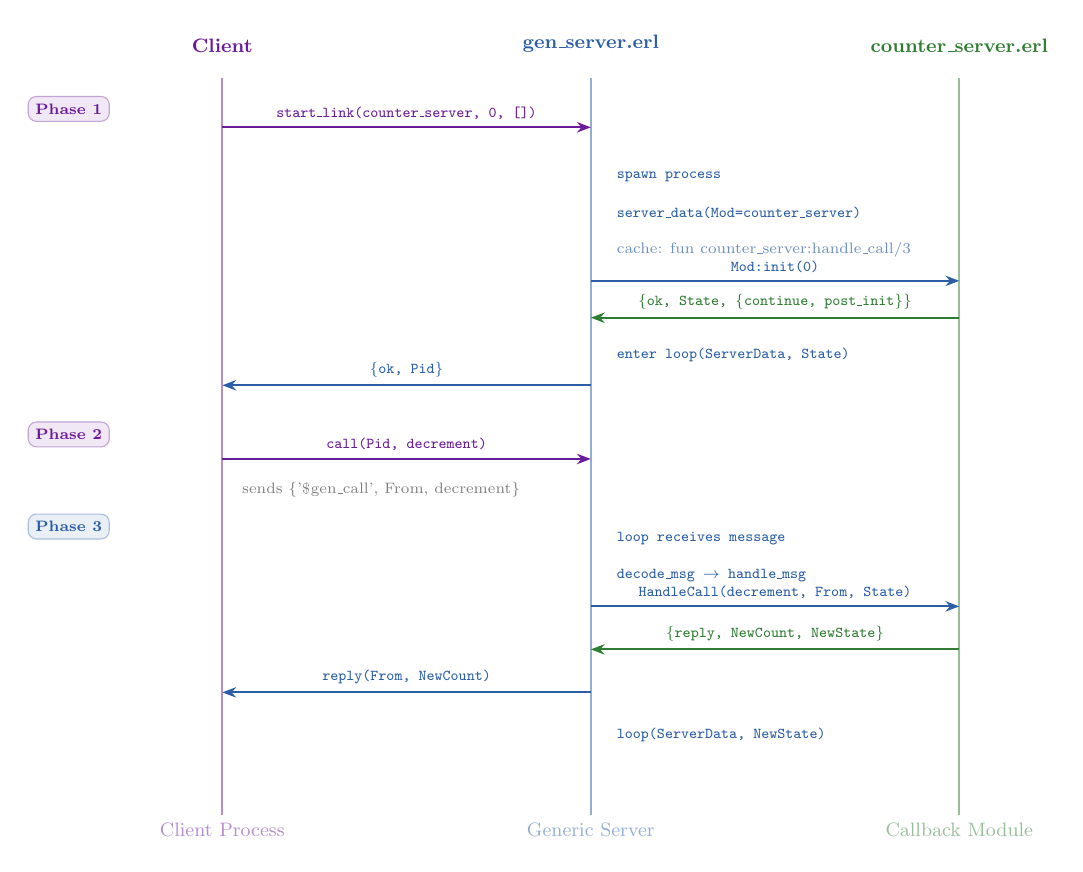
\begin{tikzpicture}[scale=0.78, every node/.style={scale=0.78},
    node distance=0.8cm,
]
    % Lifelines
    \draw[thick, erlpurple!50] (0, 0) -- (0, -12) node[below, font=\small] {Client Process};
    \draw[thick, erlblue!50] (6, 0) -- (6, -12) node[below, font=\small] {Generic Server};
    \draw[thick, erlgreen!50] (12, 0) -- (12, -12) node[below, font=\small] {Callback Module};

    % Phase 1: start_link
    \node[font=\small\bfseries\color{erlpurple}, anchor=south] at (0, 0.3) {Client};
    \node[font=\small\bfseries\color{erlblue}, anchor=south] at (6, 0.3) {gen\_server.erl};
    \node[font=\small\bfseries\color{erlgreen}, anchor=south] at (12, 0.3) {counter\_server.erl};

    % Phase label
    \node[fill=erlpurple!10, draw=erlpurple!40, rounded corners=3pt,
          font=\scriptsize\bfseries\color{erlpurple}] at (-2.5, -0.5) {Phase 1};

    \draw[-{Stealth[length=5pt]}, thick, erlpurple]
        (0, -0.8) -- node[above, font=\scriptsize\ttfamily] {start\_link(counter\_server, 0, [])} (6, -0.8);

    \node[font=\scriptsize\ttfamily, anchor=west, text=erlblue] at (6.3, -1.6) {spawn process};
    \node[font=\scriptsize\ttfamily, anchor=west, text=erlblue] at (6.3, -2.2) {server\_data(Mod=counter\_server)};
    \node[font=\scriptsize\color{erlblue!70}, anchor=west] at (6.3, -2.8) {cache: fun counter\_server:handle\_call/3};

    \draw[-{Stealth[length=5pt]}, thick, erlblue]
        (6, -3.3) -- node[above, font=\scriptsize\ttfamily] {Mod:init(0)} (12, -3.3);

    \draw[-{Stealth[length=5pt]}, thick, erlgreen]
        (12, -3.9) -- node[above, font=\scriptsize\ttfamily] {\{ok, State, \{continue, post\_init\}\}} (6, -3.9);

    \node[font=\scriptsize\ttfamily, anchor=west, text=erlblue] at (6.3, -4.5) {enter loop(ServerData, State)};

    \draw[-{Stealth[length=5pt]}, thick, erlblue]
        (6, -5.0) -- node[above, font=\scriptsize\ttfamily] {\{ok, Pid\}} (0, -5.0);

    % Phase 2: call
    \node[fill=erlpurple!10, draw=erlpurple!40, rounded corners=3pt,
          font=\scriptsize\bfseries\color{erlpurple}] at (-2.5, -5.8) {Phase 2};

    \draw[-{Stealth[length=5pt]}, thick, erlpurple]
        (0, -6.2) -- node[above, font=\scriptsize\ttfamily] {call(Pid, decrement)} (6, -6.2);

    \node[font=\scriptsize\color{gray}, anchor=west] at (0.2, -6.7) {sends \{'\$gen\_call', From, decrement\}};

    % Phase 3: dispatch
    \node[fill=erlblue!10, draw=erlblue!40, rounded corners=3pt,
          font=\scriptsize\bfseries\color{erlblue}] at (-2.5, -7.3) {Phase 3};

    \node[font=\scriptsize\ttfamily, anchor=west, text=erlblue] at (6.3, -7.5) {loop receives message};
    \node[font=\scriptsize\ttfamily, anchor=west, text=erlblue] at (6.3, -8.1) {decode\_msg $\to$ handle\_msg};

    \draw[-{Stealth[length=5pt]}, thick, erlblue]
        (6, -8.6) -- node[above, font=\scriptsize\ttfamily] {HandleCall(decrement, From, State)} (12, -8.6);

    \draw[-{Stealth[length=5pt]}, thick, erlgreen]
        (12, -9.3) -- node[above, font=\scriptsize\ttfamily] {\{reply, NewCount, NewState\}} (6, -9.3);

    \draw[-{Stealth[length=5pt]}, thick, erlblue]
        (6, -10.0) -- node[above, font=\scriptsize\ttfamily] {reply(From, NewCount)} (0, -10.0);

    \node[font=\scriptsize\ttfamily, anchor=west, text=erlblue] at (6.3, -10.7) {loop(ServerData, NewState)};

\end{tikzpicture}
\caption{函数注册与消息分发的完整时序（对应架构图中 \ding{172}--\ding{185}）}
\label{fig:registration-sequence}
\end{figure}

\subsubsection{总结}

\begin{table}[H]
\centering
\footnotesize
\begin{tabular}{@{}cp{8.5cm}c@{}}
\toprule
\textbf{阶段} & \textbf{发生了什么} & \textbf{涉及模块名？} \\
\midrule
Phase 1 & \texttt{counter\_server} 作为参数传入，被存入 \texttt{\#server\_data.module}，同时 \texttt{fun counter\_server:handle\_call/3} 等函数引用被缓存 & \checkmark \\
\midrule
Phase 2 & 客户端只向 Pid 发送 \texttt{\{'\$gen\_call', From, decrement\}} 消息 & --- \\
\midrule
Phase 3 & 框架从 \texttt{\#server\_data} 中取出缓存的 \texttt{HandleCall} 函数引用，直接调用 \texttt{counter\_server:handle\_call/3} & \checkmark \\
\bottomrule
\end{tabular}
\caption{三个阶段中模块名的角色}
\label{tab:module-name-phases}
\end{table}

\begin{notebox}[函数式编程的核心思想]
\texttt{?MODULE} 不是在 \texttt{call} 的时候注册的，而是在 \texttt{start\_link} 的时候就已经通过
\texttt{server\_data/4} 函数把模块名和回调函数引用``绑定''到了 Server 进程的内部状态中。
之后每次收到消息，Server 进程直接从自己的 \texttt{\#server\_data} record 中取出函数引用来调用，
不需要再查找模块名。

这正是架构图中 \ding{172} 虚线箭头所表达的``函数注册''过程——
\textbf{模块名（一个原子）作为数据传递，实现了行为的延迟绑定}，
是 Erlang 函数式编程的核心思想之一。
\end{notebox}

\subsection{回调模块：counter\_server}

整篇文档使用一个极简的计数器服务器作为回调模块。它足够简单，让我们把注意力集中在 gen\_server 的 API 上，而不是业务逻辑。

\begin{lstlisting}[style=erlangstyle, caption={counter\_server.erl --- 贯穿全文的回调模块}]
-module(counter_server).
-behaviour(gen_server).

%% Client API
-export([start_link/0, start_link/1, start/0, start/1]).
-export([increment/1, decrement/1, get_count/1, reset/1]).
-export([slow_operation/2, crash/1]).

%% gen_server callbacks
-export([init/1, handle_call/3, handle_cast/2,
         handle_info/2, handle_continue/2,
         terminate/2, code_change/3, format_status/2]).

%%% ============================================================
%%% Client API (thin wrappers around gen_server library functions)
%%% ============================================================

start_link() ->
    gen_server:start_link(?MODULE, 0, []).

start_link(InitCount) ->
    gen_server:start_link(?MODULE, InitCount, []).

start() ->
    gen_server:start(?MODULE, 0, []).

start(InitCount) ->
    gen_server:start(?MODULE, InitCount, []).

increment(Server) ->
    gen_server:call(Server, increment).

decrement(Server) ->
    gen_server:call(Server, decrement).

get_count(Server) ->
    gen_server:call(Server, get_count).

reset(Server) ->
    gen_server:cast(Server, reset).

slow_operation(Server, Duration) ->
    gen_server:call(Server, {slow_op, Duration}).

crash(Server) ->
    gen_server:cast(Server, crash).

%%% ============================================================
%%% gen_server callbacks
%%% ============================================================

init(InitCount) when is_integer(InitCount) ->
    process_flag(trap_exit, true),
    io:format("[counter] init: count=~p, pid=~p~n",
              [InitCount, self()]),
    {ok, #{count => InitCount, history => []},
     {continue, post_init}};
init(_) ->
    {stop, {error, bad_init_arg}}.

handle_continue(post_init, State) ->
    io:format("[counter] post_init complete~n"),
    {noreply, State}.

handle_call(increment, _From, #{count := C} = State) ->
    NewCount = C + 1,
    {reply, NewCount, State#{count := NewCount,
        history := [{increment, NewCount} |
                    maps:get(history, State)]}};

handle_call(decrement, _From, #{count := C} = State) ->
    NewCount = C - 1,
    {reply, NewCount, State#{count := NewCount,
        history := [{decrement, NewCount} |
                    maps:get(history, State)]}};

handle_call(get_count, _From, #{count := C} = State) ->
    {reply, C, State};

handle_call({slow_op, Duration}, _From, State) ->
    timer:sleep(Duration),
    {reply, {ok, done_after, Duration}, State};

handle_call(_Request, _From, State) ->
    {reply, {error, unknown_request}, State}.

handle_cast(reset, State) ->
    io:format("[counter] reset to 0~n"),
    {noreply, State#{count := 0, history := []}};

handle_cast(crash, _State) ->
    error(deliberate_crash);

handle_cast(_Msg, State) ->
    {noreply, State}.

handle_info(timeout, State) ->
    io:format("[counter] timeout fired~n"),
    {noreply, State};

handle_info({custom_msg, Payload}, State) ->
    io:format("[counter] received custom_msg: ~p~n", [Payload]),
    {noreply, State};

handle_info({'EXIT', Pid, Reason}, State) ->
    io:format("[counter] linked process ~p exited: ~p~n",
              [Pid, Reason]),
    {noreply, State};

handle_info(Info, State) ->
    io:format("[counter] unexpected info: ~p~n", [Info]),
    {noreply, State}.

terminate(Reason, #{count := C}) ->
    io:format("[counter] terminating: reason=~p, "
              "final_count=~p~n", [Reason, C]),
    ok.

code_change(_OldVsn, State, _Extra) ->
    {ok, State}.

format_status(_Opt, [_PDict, #{count := C, history := H}]) ->
    [{data, [{"State",
              #{count => C,
                history_length => length(H)}}]}].
\end{lstlisting}

\begin{tipbox}[设计要点]
\begin{itemize}[leftmargin=1.5em]
    \item 所有客户端 API 都是对 \texttt{gen\_server:call/2,3} 和 \texttt{gen\_server:cast/2} 的薄封装
    \item \texttt{init/1} 设置了 \texttt{trap\_exit}，并使用 \texttt{\{continue, post\_init\}} 演示 handle\_continue
    \item \texttt{slow\_operation} 用于演示超时场景
    \item \texttt{crash} 用于演示错误处理
    \item \texttt{format\_status} 隐藏了完整的 history 列表
\end{itemize}
\end{tipbox}


% ============================================================
% Section 2: Starting and Stopping
% ============================================================
\section{启动与停止}

\subsection{gen\_server:start\_link/3,4 --- 链接启动}

\begin{figure}[H]
\centering
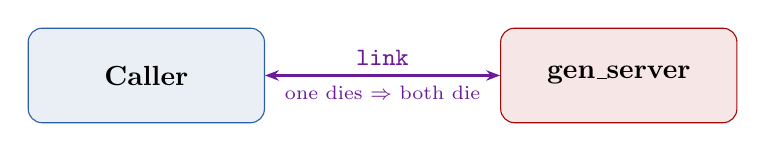
\begin{tikzpicture}[
    box/.style={draw=#1, fill=#1!10, rounded corners=5pt,
                minimum width=3cm, minimum height=1.2cm, font=\bfseries},
]
    \node[box=erlblue] (caller) at (0, 0) {Caller};
    \node[box=erlred] (gs) at (6, 0) {gen\_server};

    \draw[thick, erlpurple, {Stealth[length=5pt]}-{Stealth[length=5pt]}]
        (caller.east) -- node[above, font=\small\ttfamily] {link}
                         node[below, font=\scriptsize\color{gray}] {one dies $\Rightarrow$ both die} (gs.west);
\end{tikzpicture}
\caption{start\_link 创建双向链接}
\end{figure}

\begin{lstlisting}[style=erlangstyle, caption={start\_link 函数签名}]
%% Without name registration (anonymous)
gen_server:start_link(Module, Args, Options) ->
    {ok, Pid} | ignore | {error, Reason}.

%% With name registration
gen_server:start_link(ServerName, Module, Args, Options) ->
    {ok, Pid} | ignore | {error, Reason}.

%% ServerName types:
%%   {local, Name}       - register locally
%%   {global, Name}      - register globally
%%   {via, RegMod, Name} - register via custom registry
\end{lstlisting}

\textbf{Shell 演示：}

\begin{lstlisting}[style=shellstyle, caption={start\_link 交互演示}]
1> c(counter_server).
{ok,counter_server}

%% Anonymous start (no name registration)
2> {ok, Pid1} = gen_server:start_link(counter_server, 0, []).
[counter] init: count=0, pid=<0.89.0>
[counter] post_init complete
{ok,<0.89.0>}

%% Local name registration
3> {ok, Pid2} = gen_server:start_link(
       {local, my_counter}, counter_server, 100, []).
[counter] init: count=100, pid=<0.91.0>
[counter] post_init complete
{ok,<0.91.0>}

%% Duplicate name fails
4> gen_server:start_link({local, my_counter}, counter_server, 0, []).
{error,{already_started,<0.91.0>}}
\end{lstlisting}

\begin{warnbox}[Shell 中 start\_link 的陷阱]
在 Shell 中使用 \texttt{start\_link} 时，Shell 进程与 gen\_server 进程是链接的。如果 gen\_server 崩溃，Shell 进程也会崩溃并重启，导致 \texttt{self()} 返回新的 PID。开发测试时建议使用 \texttt{start}。
\end{warnbox}

\subsection{gen\_server:start/3,4 --- 非链接启动}

\begin{lstlisting}[style=shellstyle, caption={start 交互演示}]
%% No link - server and caller are independent
5> {ok, Pid3} = gen_server:start(counter_server, 0, []).
[counter] init: count=0, pid=<0.95.0>
[counter] post_init complete
{ok,<0.95.0>}

%% Server crash does NOT affect shell
6> counter_server:crash(Pid3).
ok
7> self().
<0.85.0>   %% Shell PID unchanged!
\end{lstlisting}

\subsection{gen\_server:start\_monitor/3,4 --- 监控启动 (OTP 23+)}

\begin{lstlisting}[style=erlangstyle, caption={start\_monitor 函数签名}]
gen_server:start_monitor(Module, Args, Options) ->
    {ok, {Pid, MonRef}} | ignore | {error, Reason}.

gen_server:start_monitor(ServerName, Module, Args, Options) ->
    {ok, {Pid, MonRef}} | ignore | {error, Reason}.
\end{lstlisting}

\begin{lstlisting}[style=shellstyle, caption={start\_monitor 交互演示}]
8> {ok, {Pid4, MonRef}} = gen_server:start_monitor(
       counter_server, 0, []).
[counter] init: count=0, pid=<0.100.0>
[counter] post_init complete
{ok,{<0.100.0>,#Ref<0.1234.5.6>}}

%% When server dies, we get a DOWN message (not EXIT)
9> counter_server:crash(Pid4).
ok
10> flush().
Shell got {'DOWN',#Ref<0.1234.5.6>,process,<0.100.0>,
           {deliberate_crash,...}}
ok
\end{lstlisting}

\begin{figure}[H]
\centering
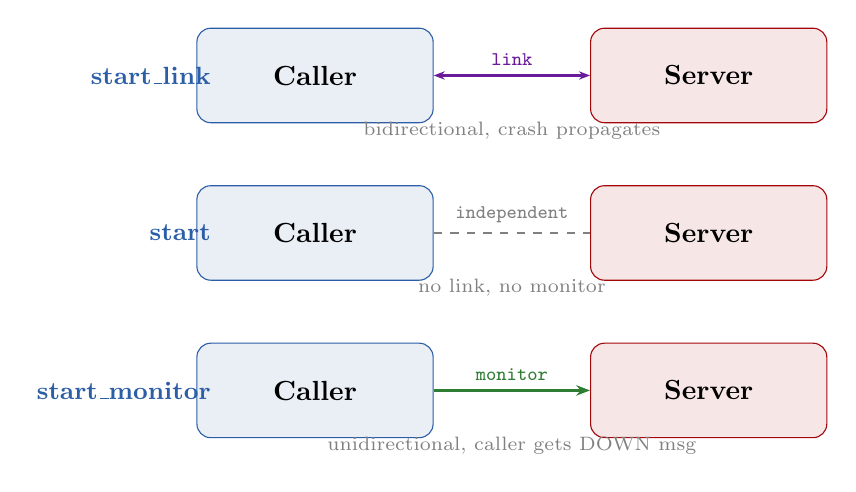
\begin{tikzpicture}[
    box/.style={draw=#1, fill=#1!10, rounded corners=5pt,
                minimum width=3cm, minimum height=1.2cm, font=\bfseries},
    arr/.style={-{Stealth[length=5pt]}, thick, #1},
]
    % start_link
    \node[box=erlblue] (c1) at (0, 2) {Caller};
    \node[box=erlred] (s1) at (5, 2) {Server};
    \draw[thick, erlpurple, {Stealth[length=4pt]}-{Stealth[length=4pt]}]
        (c1) -- node[above, font=\scriptsize\ttfamily] {link} (s1);
    \node[font=\scriptsize\color{gray}] at (2.5, 1.3) {bidirectional, crash propagates};
    \node[font=\small\bfseries\color{erlblue}, anchor=east] at (-1.2, 2) {start\_link};

    % start
    \node[box=erlblue] (c2) at (0, 0) {Caller};
    \node[box=erlred] (s2) at (5, 0) {Server};
    \draw[thick, gray, dashed] (c2) -- node[above, font=\scriptsize\ttfamily] {independent} (s2);
    \node[font=\scriptsize\color{gray}] at (2.5, -0.7) {no link, no monitor};
    \node[font=\small\bfseries\color{erlblue}, anchor=east] at (-1.2, 0) {start};

    % start_monitor
    \node[box=erlblue] (c3) at (0, -2) {Caller};
    \node[box=erlred] (s3) at (5, -2) {Server};
    \draw[arr=erlgreen] (c3) -- node[above, font=\scriptsize\ttfamily] {monitor} (s3);
    \node[font=\scriptsize\color{gray}] at (2.5, -2.7) {unidirectional, caller gets DOWN msg};
    \node[font=\small\bfseries\color{erlblue}, anchor=east] at (-1.2, -2) {start\_monitor};
\end{tikzpicture}
\caption{三种启动方式的进程关系对比}
\label{fig:start-comparison}
\end{figure}

\subsection{Options 参数详解}

\begin{lstlisting}[style=erlangstyle, caption={Options 参数}]
Options = [Option]
Option = {timeout, Timeout}       %% init/1 must return within Timeout ms
       | {debug, DebugOpts}       %% sys debug options
       | {hibernate_after, Ms}    %% auto-hibernate after Ms ms idle
       | {spawn_opt, SpawnOpts}   %% erlang:spawn_opt options
\end{lstlisting}

\begin{lstlisting}[style=shellstyle, caption={使用 Options}]
%% Start with debug tracing enabled
11> {ok, Pid5} = gen_server:start(
        {local, traced}, counter_server, 0,
        [{debug, [trace]}]).
[counter] init: count=0, pid=<0.105.0>
[counter] post_init complete
{ok,<0.105.0>}

12> gen_server:call(traced, increment).
*DBG* traced got call increment from <0.85.0>
*DBG* traced sent 1 to <0.85.0>, new state ...
1

%% Start with hibernate_after (auto-hibernate when idle)
13> {ok, Pid6} = gen_server:start(
        counter_server, 0,
        [{hibernate_after, 5000}]).
\end{lstlisting}

\subsection{gen\_server:stop/1,3 --- 优雅停止}

\begin{lstlisting}[style=erlangstyle, caption={stop 函数签名}]
gen_server:stop(ServerRef) -> ok.
%% Equivalent to stop(ServerRef, normal, infinity)

gen_server:stop(ServerRef, Reason, Timeout) -> ok.
%% Calls terminate(Reason, State) then exits
\end{lstlisting}

\begin{lstlisting}[style=shellstyle, caption={stop 交互演示}]
14> {ok, Pid7} = gen_server:start(counter_server, 42, []).
[counter] init: count=42, pid=<0.110.0>
[counter] post_init complete
{ok,<0.110.0>}

15> gen_server:call(Pid7, get_count).
42

16> gen_server:stop(Pid7).
[counter] terminating: reason=normal, final_count=42
ok

%% Process is gone
17> gen_server:call(Pid7, get_count).
** exception exit: {noproc,...}

%% Stop with custom reason and timeout
18> {ok, Pid8} = gen_server:start(counter_server, 0, []).
19> gen_server:stop(Pid8, shutdown, 5000).
[counter] terminating: reason=shutdown, final_count=0
ok
\end{lstlisting}

\begin{figure}[H]
\centering
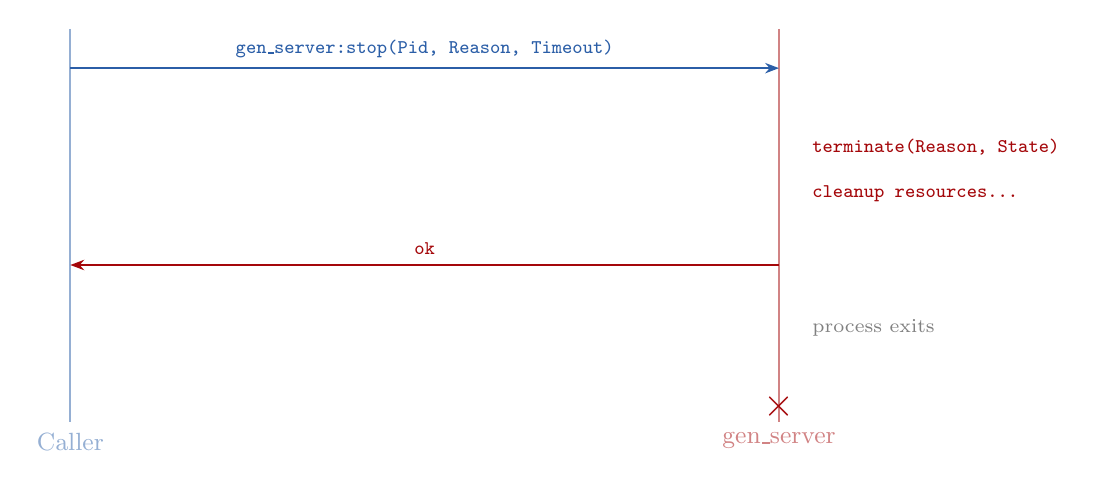
\begin{tikzpicture}[
    node distance=0.8cm,
]
    \draw[thick, erlblue!50] (0, 0) -- (0, -5) node[below, font=\small] {Caller};
    \draw[thick, erlred!50] (9, 0) -- (9, -5) node[below, font=\small] {gen\_server};

    \draw[-{Stealth[length=5pt]}, thick, erlblue]
        (0, -0.5) -- node[above, font=\scriptsize\ttfamily] {gen\_server:stop(Pid, Reason, Timeout)} (9, -0.5);

    \node[font=\scriptsize\ttfamily, anchor=west, text=erlred] at (9.3, -1.5) {terminate(Reason, State)};
    \node[font=\scriptsize\ttfamily, anchor=west, text=erlred] at (9.3, -2.1) {cleanup resources...};

    \draw[-{Stealth[length=5pt]}, thick, erlred]
        (9, -3) -- node[above, font=\scriptsize\ttfamily] {ok} (0, -3);

    \node[font=\scriptsize\color{gray}, anchor=west] at (9.3, -3.8) {process exits};
    \draw[thick, erlred!50, dashed] (9, -3.5) -- (9, -4.5);
    \node[font=\Large\color{erlred}] at (9, -4.8) {$\times$};
\end{tikzpicture}
\caption{gen\_server:stop 的执行流程}
\label{fig:stop-flow}
\end{figure}


% ============================================================
% Section 3: Synchronous Call
% ============================================================
\section{同步调用：gen\_server:call/2,3}

\subsection{基本用法}

\begin{lstlisting}[style=erlangstyle, caption={call 函数签名}]
gen_server:call(ServerRef, Request) -> Reply.
%% Default timeout: 5000ms (5 seconds)

gen_server:call(ServerRef, Request, Timeout) -> Reply.
%% Timeout = integer() >= 0 | infinity
\end{lstlisting}

\begin{lstlisting}[style=shellstyle, caption={call 基本交互}]
1> {ok, Pid} = gen_server:start(counter_server, 0, []).
{ok,<0.89.0>}

2> gen_server:call(Pid, increment).
1
3> gen_server:call(Pid, increment).
2
4> gen_server:call(Pid, get_count).
2
5> gen_server:call(Pid, decrement).
1
\end{lstlisting}

\subsection{ServerRef 的多种形式}

\begin{lstlisting}[style=shellstyle, caption={不同的 ServerRef 形式}]
%% By PID
6> gen_server:call(Pid, get_count).
1

%% By local name
7> {ok, _} = gen_server:start(
       {local, ctr}, counter_server, 0, []).
8> gen_server:call(ctr, increment).
1

%% By {Name, Node} for remote node
9> gen_server:call({ctr, 'node1@host'}, get_count).

%% By {global, Name}
10> gen_server:call({global, global_ctr}, get_count).

%% By {via, Module, Name}
11> gen_server:call({via, gproc, {n, l, my_ctr}}, get_count).
\end{lstlisting}

\begin{figure}[H]
\centering
\begin{tikzpicture}[
    ref/.style={draw=erlblue, fill=erlblue!8, rounded corners=4pt,
                minimum width=5.5cm, minimum height=0.9cm, font=\small\ttfamily, align=center},
    desc/.style={font=\small, anchor=west, text width=6cm},
]
    \node[font=\large\bfseries\color{erlblue}] at (0, 4) {ServerRef 类型};

    \node[ref] (r1) at (0, 3) {pid()};
    \node[ref] (r2) at (0, 1.8) {atom()};
    \node[ref] (r3) at (0, 0.6) {\{Name :: atom(), Node :: node()\}};
    \node[ref] (r4) at (0, -0.6) {\{global, GlobalName :: term()\}};
    \node[ref] (r5) at (0, -1.8) {\{via, RegMod :: module(), ViaName\}};

    \node[desc] at (3.5, 3) {直接使用进程 PID};
    \node[desc] at (3.5, 1.8) {本地注册名（当前节点）};
    \node[desc] at (3.5, 0.6) {远程节点上的本地注册名};
    \node[desc] at (3.5, -0.6) {全局注册名（跨所有连接节点）};
    \node[desc] at (3.5, -1.8) {自定义注册模块（如 gproc）};
\end{tikzpicture}
\caption{ServerRef 的五种形式}
\label{fig:server-ref-types}
\end{figure}

\subsection{超时控制}

\begin{lstlisting}[style=shellstyle, caption={call 超时演示}]
%% slow_operation sleeps for Duration ms
%% Default 5s timeout - this will succeed
12> gen_server:call(Pid, {slow_op, 1000}).
{ok,done_after,1000}

%% Custom short timeout - this will fail
13> gen_server:call(Pid, {slow_op, 3000}, 1000).
** exception exit: {timeout,{gen_server,call,[<0.89.0>,...]}}

%% Infinite timeout - never times out
14> gen_server:call(Pid, {slow_op, 3000}, infinity).
{ok,done_after,3000}
\end{lstlisting}

\begin{warnbox}[超时后的行为]
当 \texttt{call} 超时时：
\begin{itemize}[leftmargin=1.5em]
    \item \textbf{客户端}：抛出 \texttt{exit:\{timeout, ...\}} 异常
    \item \textbf{服务器}：\textbf{继续运行}，仍在处理该请求
    \item 服务器处理完后的回复会变成客户端消息队列中的"残留消息"
\end{itemize}
\end{warnbox}

\begin{figure}[H]
\centering
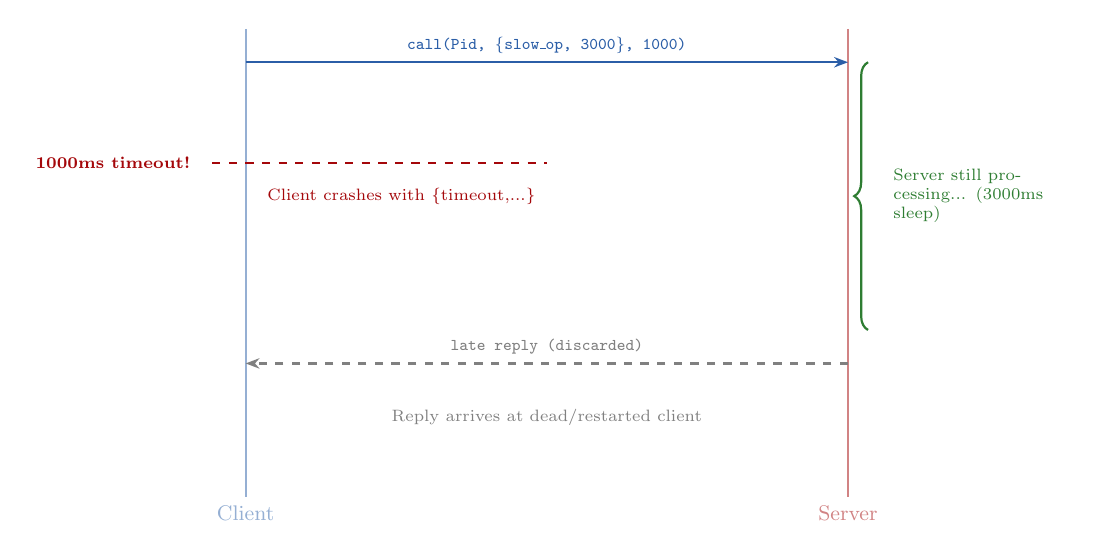
\begin{tikzpicture}[scale=0.85, every node/.style={scale=0.85},
    node distance=0.8cm,
]
    \draw[thick, erlblue!50] (0, 0) -- (0, -7) node[below, font=\small] {Client};
    \draw[thick, erlred!50] (9, 0) -- (9, -7) node[below, font=\small] {Server};

    % call
    \draw[-{Stealth[length=5pt]}, thick, erlblue]
        (0, -0.5) -- node[above, font=\scriptsize\ttfamily] {call(Pid, \{slow\_op, 3000\}, 1000)} (9, -0.5);

    % timeout line
    \draw[dashed, erlred, thick] (-0.5, -2) -- (4.5, -2);
    \node[font=\scriptsize\bfseries\color{erlred}, anchor=east] at (-0.7, -2) {1000ms timeout!};
    \node[font=\scriptsize\color{erlred}, anchor=west] at (0.2, -2.5) {Client crashes with \{timeout,...\}};

    % Server still working
    \draw[thick, erlgreen, decorate, decoration={brace, amplitude=5pt, mirror}]
        (9.3, -0.5) -- (9.3, -4.5)
        node[midway, right=6pt, font=\scriptsize, text width=2.5cm] {Server still processing... (3000ms sleep)};

    % Late reply
    \draw[-{Stealth[length=5pt]}, thick, gray, dashed]
        (9, -5) -- node[above, font=\scriptsize\ttfamily\color{gray}] {late reply (discarded)} (0, -5);

    \node[font=\scriptsize\color{gray}] at (4.5, -5.8) {Reply arrives at dead/restarted client};
\end{tikzpicture}
\caption{call 超时后的时序：服务器继续运行，回复变成残留消息}
\label{fig:call-timeout}
\end{figure}

\subsection{call 失败的各种原因}

\begin{table}[H]
\centering
\small
\begin{tabular}{@{}lp{8cm}@{}}
\toprule
\textbf{exit reason} & \textbf{说明} \\
\midrule
\texttt{\{timeout, \{gen\_server, call, ...\}\}} & 服务器在 Timeout 内未回复 \\
\texttt{\{noproc, ...\}} & 服务器进程不存在 \\
\texttt{\{nodedown, Node\}} & 远程节点断开连接 \\
\texttt{\{normal, ...\}} & 服务器在处理请求时正常退出 \\
\texttt{\{shutdown, ...\}} & 服务器被 supervisor 关闭 \\
\texttt{\{calling\_self, ...\}} & 试图 call 自己（死锁检测） \\
\bottomrule
\end{tabular}
\caption{gen\_server:call 可能的 exit 原因}
\label{tab:call-exit-reasons}
\end{table}


% ============================================================
% Section 4: Asynchronous Cast
% ============================================================
\section{异步调用：gen\_server:cast/2}

\subsection{基本用法}

\begin{lstlisting}[style=erlangstyle, caption={cast 函数签名}]
gen_server:cast(ServerRef, Request) -> ok.
%% Always returns ok immediately, even if server doesn't exist!
\end{lstlisting}

\begin{lstlisting}[style=shellstyle, caption={cast 交互演示}]
1> {ok, Pid} = gen_server:start(counter_server, 10, []).
{ok,<0.89.0>}

%% cast returns ok immediately
2> gen_server:cast(Pid, reset).
[counter] reset to 0
ok

3> gen_server:call(Pid, get_count).
0

%% cast to non-existent process - still returns ok!
4> gen_server:cast(self(), some_msg).
ok
\end{lstlisting}

\begin{figure}[H]
\centering
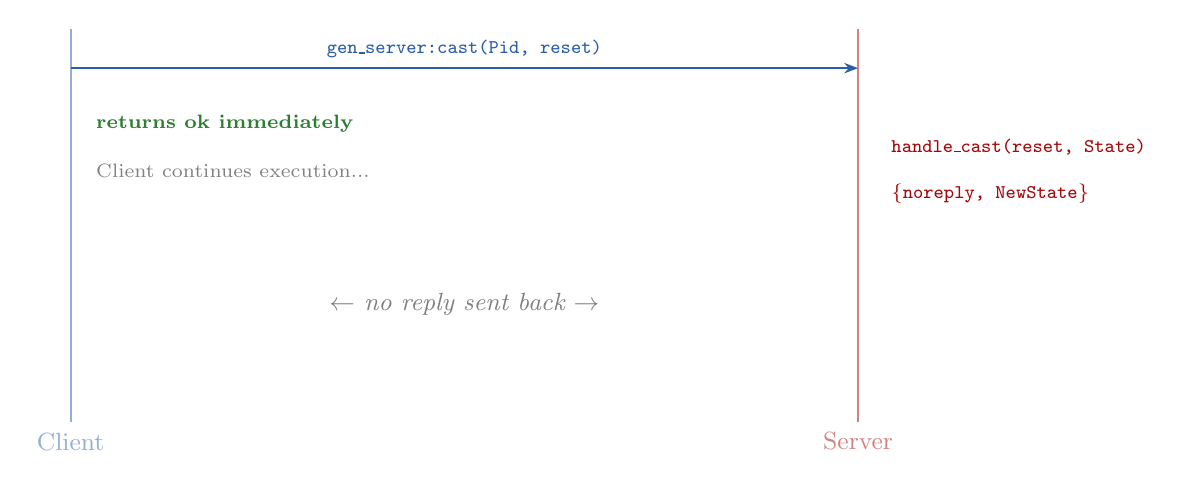
\begin{tikzpicture}[
    node distance=0.8cm,
]
    \draw[thick, erlblue!50] (0, 0) -- (0, -5) node[below, font=\small] {Client};
    \draw[thick, erlred!50] (10, 0) -- (10, -5) node[below, font=\small] {Server};

    % cast
    \draw[-{Stealth[length=5pt]}, thick, erlblue]
        (0, -0.5) -- node[above, font=\scriptsize\ttfamily] {gen\_server:cast(Pid, reset)} (10, -0.5);

    % ok returned immediately
    \node[font=\scriptsize\bfseries\color{erlgreen}, anchor=west] at (0.2, -1.2) {returns ok immediately};
    \node[font=\scriptsize\color{gray}, anchor=west] at (0.2, -1.8) {Client continues execution...};

    % Server processes
    \node[font=\scriptsize\ttfamily, anchor=west, text=erlred] at (10.3, -1.5) {handle\_cast(reset, State)};
    \node[font=\scriptsize\ttfamily, anchor=west, text=erlred] at (10.3, -2.1) {\{noreply, NewState\}};

    % No reply arrow
    \node[font=\small\itshape\color{gray}] at (5, -3.5) {$\leftarrow$ no reply sent back $\rightarrow$};
\end{tikzpicture}
\caption{cast 是 fire-and-forget：发送后立即返回，无回复}
\label{fig:cast-flow}
\end{figure}

\subsection{call vs cast 选择指南}

\begin{table}[H]
\centering
\begin{tabular}{@{}lcc@{}}
\toprule
\textbf{特性} & \textbf{call} & \textbf{cast} \\
\midrule
阻塞客户端 & $\checkmark$ & --- \\
有返回值 & $\checkmark$ & 始终返回 \texttt{ok} \\
确认送达 & $\checkmark$ & --- \\
背压（back-pressure） & $\checkmark$ & --- \\
可能超时 & $\checkmark$ & --- \\
服务器不存在时 & 抛异常 & 静默返回 \texttt{ok} \\
\bottomrule
\end{tabular}
\caption{call vs cast 对比}
\label{tab:call-vs-cast}
\end{table}

\begin{tipbox}[何时用 cast？]
\begin{itemize}[leftmargin=1.5em]
    \item 不需要返回值的通知类操作（如日志、统计）
    \item 不需要确认的 fire-and-forget 场景
    \item 需要避免客户端阻塞时
\end{itemize}
\textbf{注意}：cast 没有背压机制，如果发送速度远大于处理速度，服务器的消息队列会无限增长！
\end{tipbox}


% ============================================================
% Section 5: Explicit Reply
% ============================================================
\section{显式回复：gen\_server:reply/2}

\subsection{为什么需要显式回复？}

通常 \texttt{handle\_call} 通过返回 \texttt{\{reply, Reply, NewState\}} 来回复客户端。但有时你需要：
\begin{itemize}[leftmargin=2em]
    \item 先回复客户端，再做耗时的后续操作
    \item 在另一个进程中回复
    \item 根据条件决定是否回复
\end{itemize}

\begin{lstlisting}[style=erlangstyle, caption={reply 函数签名}]
gen_server:reply(Client, Reply) -> ok.
%% Client = From argument from handle_call/3
%% From = {Pid, Tag}
\end{lstlisting}

\subsection{示例：先回复，再做后续工作}

\begin{lstlisting}[style=erlangstyle, caption={在 handle\_call 中使用 reply/2}]
%% In callback module:
handle_call({allocate, Pid}, From, State) ->
    {NewState, Reply} = do_allocate(State, Pid),

    %% Reply immediately - client unblocks now
    gen_server:reply(From, Reply),

    %% Do slow post-processing (client already got response)
    log_allocation(Pid, Reply),
    notify_monitors(NewState),

    %% Return noreply since we already replied manually
    {noreply, NewState}.
\end{lstlisting}

\begin{figure}[H]
\centering
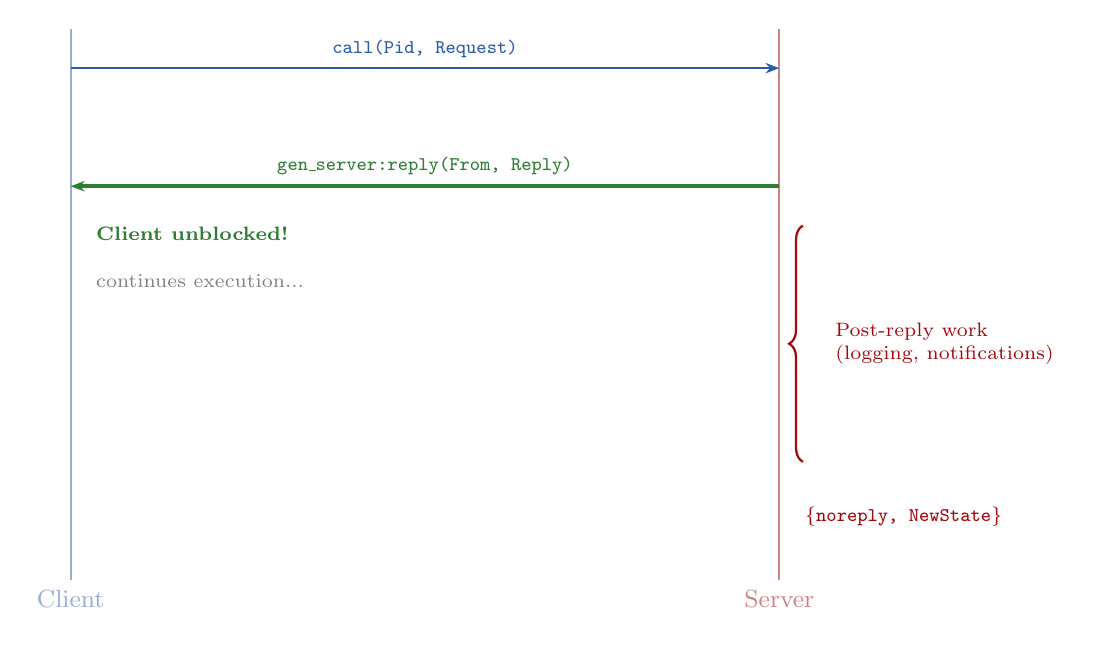
\begin{tikzpicture}[
    node distance=0.8cm,
]
    \draw[thick, erlblue!50] (0, 0) -- (0, -7) node[below, font=\small] {Client};
    \draw[thick, erlred!50] (9, 0) -- (9, -7) node[below, font=\small] {Server};

    % call
    \draw[-{Stealth[length=5pt]}, thick, erlblue]
        (0, -0.5) -- node[above, font=\scriptsize\ttfamily] {call(Pid, Request)} (9, -0.5);

    % explicit reply (early)
    \draw[-{Stealth[length=5pt]}, thick, erlgreen, line width=1.5pt]
        (9, -2) -- node[above, font=\scriptsize\ttfamily\color{erlgreen}] {gen\_server:reply(From, Reply)} (0, -2);

    \node[font=\scriptsize\bfseries\color{erlgreen}, anchor=west] at (0.2, -2.6) {Client unblocked!};
    \node[font=\scriptsize\color{gray}, anchor=west] at (0.2, -3.2) {continues execution...};

    % Server post-work
    \draw[thick, erlred, decorate, decoration={brace, amplitude=5pt, mirror}]
        (9.3, -2.5) -- (9.3, -5.5)
        node[midway, right=8pt, font=\scriptsize, text width=3cm] {Post-reply work\\(logging, notifications)};

    \node[font=\scriptsize\ttfamily\color{erlred}, anchor=west] at (9.2, -6.2) {\{noreply, NewState\}};
\end{tikzpicture}
\caption{显式回复：客户端提前解除阻塞}
\label{fig:explicit-reply-flow}
\end{figure}

\subsection{示例：委托给另一个进程回复}

\begin{lstlisting}[style=erlangstyle, caption={委托回复}]
handle_call({compute, Data}, From, State) ->
    %% Spawn a worker to do heavy computation
    spawn(fun() ->
        Result = heavy_computation(Data),
        %% Worker replies on behalf of the server
        gen_server:reply(From, Result)
    end),
    %% Server is free to handle next message
    {noreply, State}.
\end{lstlisting}


% ============================================================
% Section 6: Asynchronous Request
% ============================================================
\section{异步请求：gen\_server:send\_request (OTP 23+)}

\subsection{动机}

\texttt{call} 是阻塞的，\texttt{cast} 没有返回值。\texttt{send\_request} 提供了第三种选择：\textbf{非阻塞地发送请求，稍后收取回复}。

\begin{figure}[H]
\centering
\begin{tikzpicture}[
    style/.style={draw=#1, fill=#1!8, rounded corners=6pt,
                  minimum width=4cm, minimum height=1.5cm, text width=3.5cm, align=center, font=\small},
]
    \node[style=erlblue] (call) at (0, 0) {\textbf{call}\\阻塞等待回复};
    \node[style=erlgreen] (cast) at (5, 0) {\textbf{cast}\\无回复};
    \node[style=erlpurple] (sr) at (10, 0) {\textbf{send\_request}\\非阻塞，稍后取回复};

    \node[font=\scriptsize\color{gray}] at (0, -1.3) {同步};
    \node[font=\scriptsize\color{gray}] at (5, -1.3) {异步 (fire \& forget)};
    \node[font=\scriptsize\color{gray}] at (10, -1.3) {异步 (有回复)};
\end{tikzpicture}
\caption{三种请求模式对比}
\label{fig:three-modes}
\end{figure}

\subsection{send\_request/2 + receive\_response/2}

\begin{lstlisting}[style=erlangstyle, caption={send\_request 函数签名}]
gen_server:send_request(ServerRef, Request) -> ReqId.

%% Later, collect the reply:
gen_server:receive_response(ReqId, Timeout) ->
    {reply, Reply} | timeout | {error, {Reason, ServerRef}}.

gen_server:wait_response(ReqId, Timeout) ->
    {reply, Reply} | timeout | {error, {Reason, ServerRef}}.

gen_server:check_response(Msg, ReqId) ->
    {reply, Reply} | no_reply | {error, {Reason, ServerRef}}.
\end{lstlisting}

\begin{lstlisting}[style=shellstyle, caption={send\_request 交互演示}]
1> {ok, Pid} = gen_server:start(counter_server, 0, []).
{ok,<0.89.0>}

%% Send request without blocking
2> ReqId = gen_server:send_request(Pid, increment).
#Ref<0.1234.5.6>

%% Do other work here...
3> io:format("I'm not blocked!~n").
I'm not blocked!
ok

%% Now collect the reply
4> gen_server:receive_response(ReqId, 5000).
{reply,1}

%% Or use wait_response (same but returns 'timeout' atom)
5> ReqId2 = gen_server:send_request(Pid, increment).
6> gen_server:wait_response(ReqId2, 1000).
{reply,2}
\end{lstlisting}

\subsection{send\_request/4 + 请求集合 (OTP 25+)}

当需要同时向多个服务器发送请求时，可以使用请求集合：

\begin{lstlisting}[style=erlangstyle, caption={请求集合用法}]
%% Create a request ID collection
ReqIdCol0 = gen_server:reqids_new(),

%% Send requests to multiple servers, collecting IDs
ReqIdCol1 = gen_server:send_request(
    Server1, get_count, server1, ReqIdCol0),
ReqIdCol2 = gen_server:send_request(
    Server2, get_count, server2, ReqIdCol1),
ReqIdCol3 = gen_server:send_request(
    Server3, get_count, server3, ReqIdCol2),

%% Receive responses one by one
{reply, Reply1, Label1, ReqIdCol4} =
    gen_server:receive_response(ReqIdCol3, 5000),
{reply, Reply2, Label2, ReqIdCol5} =
    gen_server:receive_response(ReqIdCol4, 5000),
{reply, Reply3, Label3, _ReqIdCol6} =
    gen_server:receive_response(ReqIdCol5, 5000).
\end{lstlisting}

\begin{lstlisting}[style=shellstyle, caption={请求集合交互演示}]
1> {ok, S1} = gen_server:start(counter_server, 10, []).
2> {ok, S2} = gen_server:start(counter_server, 20, []).
3> {ok, S3} = gen_server:start(counter_server, 30, []).

%% Build request collection
4> C0 = gen_server:reqids_new().
5> C1 = gen_server:send_request(S1, get_count, s1, C0).
6> C2 = gen_server:send_request(S2, get_count, s2, C1).
7> C3 = gen_server:send_request(S3, get_count, s3, C2).

%% How many pending requests?
8> gen_server:reqids_size(C3).
3

%% Collect replies (order depends on which server replies first)
9> {reply, R1, Label1, C4} = gen_server:receive_response(C3, 5000).
{reply,10,s1,...}
10> {reply, R2, Label2, C5} = gen_server:receive_response(C4, 5000).
{reply,20,s2,...}
11> {reply, R3, Label3, C6} = gen_server:receive_response(C5, 5000).
{reply,30,s3,...}
\end{lstlisting}

\begin{figure}[H]
\centering
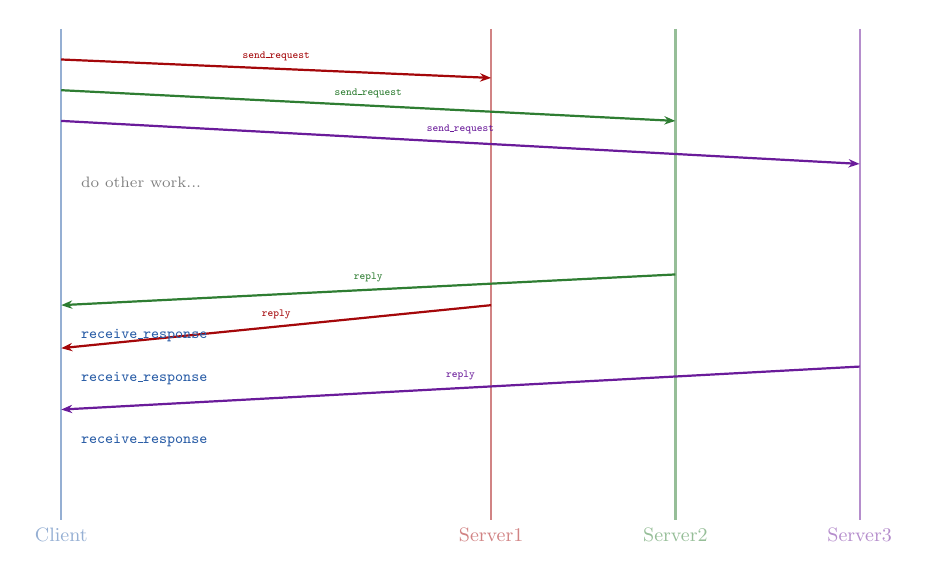
\begin{tikzpicture}[scale=0.78, every node/.style={scale=0.78},
    node distance=0.5cm,
]
    \draw[thick, erlblue!50] (0, 0) -- (0, -8) node[below, font=\small] {Client};
    \draw[thick, erlred!50] (7, 0) -- (7, -8) node[below, font=\small] {Server1};
    \draw[thick, erlgreen!50] (10, 0) -- (10, -8) node[below, font=\small] {Server2};
    \draw[thick, erlpurple!50] (13, 0) -- (13, -8) node[below, font=\small] {Server3};

    % Send all requests (non-blocking)
    \draw[-{Stealth[length=4pt]}, thick, erlred]
        (0, -0.5) -- node[above, font=\tiny\ttfamily] {send\_request} (7, -0.8);
    \draw[-{Stealth[length=4pt]}, thick, erlgreen]
        (0, -1.0) -- node[above, font=\tiny\ttfamily] {send\_request} (10, -1.5);
    \draw[-{Stealth[length=4pt]}, thick, erlpurple]
        (0, -1.5) -- node[above, font=\tiny\ttfamily] {send\_request} (13, -2.2);

    % Client does other work
    \node[font=\scriptsize\color{gray}, anchor=west] at (0.2, -2.5) {do other work...};

    % Replies come back
    \draw[-{Stealth[length=4pt]}, thick, erlgreen]
        (10, -4) -- node[above, font=\tiny\ttfamily] {reply} (0, -4.5);
    \draw[-{Stealth[length=4pt]}, thick, erlred]
        (7, -4.5) -- node[above, font=\tiny\ttfamily] {reply} (0, -5.2);
    \draw[-{Stealth[length=4pt]}, thick, erlpurple]
        (13, -5.5) -- node[above, font=\tiny\ttfamily] {reply} (0, -6.2);

    % receive_response calls
    \node[font=\scriptsize\ttfamily\color{erlblue}, anchor=west] at (0.2, -5) {receive\_response};
    \node[font=\scriptsize\ttfamily\color{erlblue}, anchor=west] at (0.2, -5.7) {receive\_response};
    \node[font=\scriptsize\ttfamily\color{erlblue}, anchor=west] at (0.2, -6.7) {receive\_response};
\end{tikzpicture}
\caption{send\_request 并行请求多个服务器}
\label{fig:send-request-parallel}
\end{figure}

\subsection{receive\_response vs wait\_response vs check\_response}

\begin{table}[H]
\centering
\small
\begin{tabular}{@{}lp{3.5cm}p{3.5cm}p{3.5cm}@{}}
\toprule
 & \textbf{receive\_response} & \textbf{wait\_response} & \textbf{check\_response} \\
\midrule
阻塞 & $\checkmark$ & $\checkmark$ & --- \\
超时返回 & \texttt{timeout} & \texttt{timeout} & N/A \\
无匹配消息 & 继续等待 & 继续等待 & 返回 \texttt{no\_reply} \\
清理残留消息 & $\checkmark$ & --- & --- \\
适用场景 & 最常用 & 需要保留消息 & 在 receive 循环中 \\
\bottomrule
\end{tabular}
\caption{三种响应收取方式对比}
\label{tab:response-functions}
\end{table}


% ============================================================
% Section 7: Multi-node Operations
% ============================================================
\section{多节点操作：multi\_call 与 abcast}

\subsection{gen\_server:multi\_call/2,3,4 --- 并行同步调用}

向多个节点上同名注册的 gen\_server 发送同步请求，并收集所有回复。

\begin{lstlisting}[style=erlangstyle, caption={multi\_call 函数签名}]
gen_server:multi_call(Name, Request) ->
    {Replies, BadNodes}.
%% Calls all connected nodes + self

gen_server:multi_call(Nodes, Name, Request) ->
    {Replies, BadNodes}.

gen_server:multi_call(Nodes, Name, Request, Timeout) ->
    {Replies, BadNodes}.

%% Replies  = [{Node, Reply}]
%% BadNodes = [Node]  (not found / no reply / timeout)
\end{lstlisting}

\begin{lstlisting}[style=shellstyle, caption={multi\_call 演示（需要多节点环境）}]
%% Terminal 1: Start node1
$ erl -sname node1 -setcookie demo
(node1@host)1> gen_server:start({local, ctr}, counter_server, 10, []).

%% Terminal 2: Start node2
$ erl -sname node2 -setcookie demo
(node2@host)1> gen_server:start({local, ctr}, counter_server, 20, []).

%% Terminal 3: Start node3 and call all
$ erl -sname node3 -setcookie demo
(node3@host)1> gen_server:start({local, ctr}, counter_server, 30, []).
(node3@host)2> net_adm:ping('node1@host').
pong
(node3@host)3> net_adm:ping('node2@host').
pong

%% Call all nodes at once
(node3@host)4> gen_server:multi_call(ctr, get_count).
{[{'node3@host',30},{'node1@host',10},{'node2@host',20}],[]}

%% Call specific nodes with timeout
(node3@host)5> gen_server:multi_call(
    ['node1@host', 'node2@host', 'nonexistent@host'],
    ctr, get_count, 3000).
{[{'node1@host',10},{'node2@host',20}],['nonexistent@host']}
\end{lstlisting}

\begin{figure}[H]
\centering
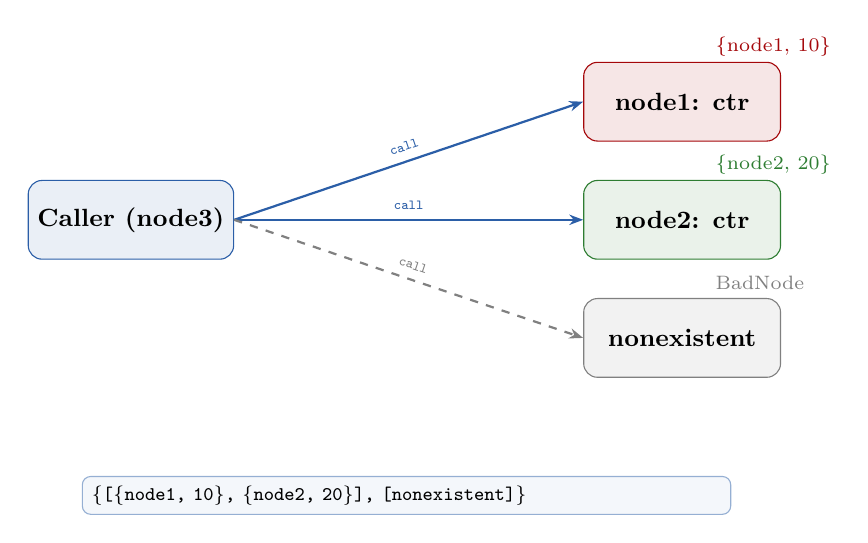
\begin{tikzpicture}[
    nd/.style={draw=#1, fill=#1!10, rounded corners=5pt,
               minimum width=2.5cm, minimum height=1cm, font=\small\bfseries},
]
    \node[nd=erlblue] (caller) at (0, 0) {Caller (node3)};

    \node[nd=erlred] (n1) at (7, 1.5) {node1: ctr};
    \node[nd=erlgreen] (n2) at (7, 0) {node2: ctr};
    \node[nd=gray] (n3) at (7, -1.5) {nonexistent};

    % Parallel calls
    \draw[-{Stealth[length=5pt]}, thick, erlblue]
        (caller.east) -- node[above, font=\tiny\ttfamily, sloped] {call} (n1.west);
    \draw[-{Stealth[length=5pt]}, thick, erlblue]
        (caller.east) -- node[above, font=\tiny\ttfamily, sloped] {call} (n2.west);
    \draw[-{Stealth[length=5pt]}, thick, gray, dashed]
        (caller.east) -- node[above, font=\tiny\ttfamily, sloped] {call} (n3.west);

    % Replies
    \node[font=\scriptsize\color{erlred}, anchor=west] at (7.3, 2.2) {\{node1, 10\}};
    \node[font=\scriptsize\color{erlgreen}, anchor=west] at (7.3, 0.7) {\{node2, 20\}};
    \node[font=\scriptsize\color{gray}, anchor=west] at (7.3, -0.8) {BadNode};

    % Result
    \node[draw=erlblue!50, fill=erlblue!5, rounded corners=3pt,
          font=\scriptsize\ttfamily, text width=8cm, align=left] at (3.5, -3.5) {
        \{[\{node1, 10\}, \{node2, 20\}], [nonexistent]\}
    };
\end{tikzpicture}
\caption{multi\_call 并行调用多个节点}
\label{fig:multi-call}
\end{figure}

\subsection{gen\_server:abcast/2,3 --- 并行异步广播}

\begin{lstlisting}[style=erlangstyle, caption={abcast 函数签名}]
gen_server:abcast(Name, Request) -> abcast.
%% Broadcasts to all connected nodes + self

gen_server:abcast(Nodes, Name, Request) -> abcast.
%% Broadcasts to specified nodes
\end{lstlisting}

\begin{lstlisting}[style=shellstyle, caption={abcast 演示}]
%% Broadcast reset to all nodes
(node3@host)6> gen_server:abcast(ctr, reset).
abcast

%% Broadcast to specific nodes
(node3@host)7> gen_server:abcast(
    ['node1@host', 'node2@host'], ctr, reset).
abcast

%% Verify all counters are reset
(node3@host)8> gen_server:multi_call(ctr, get_count).
{[{'node3@host',0},{'node1@host',0},{'node2@host',0}],[]}
\end{lstlisting}

\begin{notebox}[abcast 的特点]
\begin{itemize}[leftmargin=1.5em]
    \item 始终返回 \texttt{abcast}（不是 \texttt{ok}）
    \item 不关心节点是否存在、服务器是否注册
    \item 源码注释称之为 ``send 'n' pray''（发送然后祈祷）
    \item 触发的是 \texttt{handle\_cast/2}，不是 \texttt{handle\_call/3}
\end{itemize}
\end{notebox}

\subsection{multi\_call vs abcast 对比}

\begin{table}[H]
\centering
\begin{tabular}{@{}lcc@{}}
\toprule
\textbf{特性} & \textbf{multi\_call} & \textbf{abcast} \\
\midrule
类型 & 同步 & 异步 \\
有返回值 & $\checkmark$ (\{Replies, BadNodes\}) & 始终返回 \texttt{abcast} \\
知道哪些节点失败 & $\checkmark$ & --- \\
触发的回调 & handle\_call/3 & handle\_cast/2 \\
有超时 & $\checkmark$ & --- \\
\bottomrule
\end{tabular}
\caption{multi\_call vs abcast}
\end{table}


% ============================================================
% Section 8: Sending Raw Messages
% ============================================================
\section{发送原始消息：Pid ! Message}

\subsection{handle\_info/2 的触发}

除了 \texttt{call} 和 \texttt{cast}，任何直接用 \texttt{!} 发送给 gen\_server 进程的消息都会触发 \texttt{handle\_info/2}。

\begin{lstlisting}[style=shellstyle, caption={直接发送消息}]
1> {ok, Pid} = gen_server:start(counter_server, 0, []).
{ok,<0.89.0>}

%% Send a custom message directly
2> Pid ! {custom_msg, hello_world}.
[counter] received custom_msg: hello_world
{custom_msg,hello_world}

%% Send an unknown message
3> Pid ! some_random_atom.
[counter] unexpected info: some_random_atom
some_random_atom

%% Timer messages also go to handle_info
4> erlang:send_after(1000, Pid, {custom_msg, from_timer}).
#Ref<0.1234.5.6>
%% (1 second later)
[counter] received custom_msg: from_timer
\end{lstlisting}

\subsection{常见的 handle\_info 消息类型}

\begin{table}[H]
\centering
\small
\begin{tabular}{@{}lp{7cm}@{}}
\toprule
\textbf{消息} & \textbf{来源} \\
\midrule
\texttt{timeout} & 回调函数返回 \texttt{\{noreply, State, Timeout\}} 后超时 \\
\texttt{\{'EXIT', Pid, Reason\}} & 链接进程退出（需 \texttt{trap\_exit}） \\
\texttt{\{'DOWN', Ref, process, Pid, Reason\}} & 被监控的进程退出 \\
\texttt{\{nodedown, Node\}} & \texttt{monitor\_node} 监控的节点断开 \\
\texttt{\{tcp, Socket, Data\}} & TCP socket 数据到达 \\
\texttt{\{Ref, Result\}} & \texttt{erpc:send\_request} 的回复 \\
任意 \texttt{Pid ! Msg} & 直接发送的消息 \\
\bottomrule
\end{tabular}
\caption{常见的 handle\_info 消息类型}
\end{table}

\subsection{超时机制（Timeout）}

\begin{lstlisting}[style=erlangstyle, caption={超时机制}]
%% Set timeout in init
init(Args) ->
    {ok, State, 5000}.  %% 5 second timeout

%% Set timeout in handle_call
handle_call(Req, _From, State) ->
    {reply, ok, State, 3000}.  %% Reset timeout to 3s

%% Timeout triggers handle_info
handle_info(timeout, State) ->
    io:format("No messages for a while!~n"),
    {noreply, State, 5000}.  %% Set next timeout
\end{lstlisting}

\begin{warnbox}[超时重置规则]
\textbf{任何}到达的消息（call、cast、info）都会重置超时计时器。超时只在服务器完全空闲时触发。
\end{warnbox}


% ============================================================
% Section 9: enter_loop
% ============================================================
\section{进入循环：gen\_server:enter\_loop/3,4,5}

\subsection{动机}

有时你需要在进程启动时做复杂的初始化（比如多步骤、条件分支），\texttt{init/1} 回调不够灵活。\texttt{enter\_loop} 允许你用 \texttt{proc\_lib} 手动启动进程，完成自定义初始化后，再进入 gen\_server 的消息循环。

\begin{lstlisting}[style=erlangstyle, caption={enter\_loop 函数签名}]
gen_server:enter_loop(Module, Options, State) -> no_return().
gen_server:enter_loop(Module, Options, State, ServerName) -> no_return().
gen_server:enter_loop(Module, Options, State, ServerName, Action) ->
    no_return().

%% Action = timeout() | hibernate | {continue, Continue}
\end{lstlisting}

\subsection{示例：复杂初始化}

\begin{lstlisting}[style=erlangstyle, caption={使用 enter\_loop 的复杂初始化}]
-module(complex_init_server).
-behaviour(gen_server).
-export([start_link/1]).
-export([init/1, handle_call/3, handle_cast/2,
         handle_info/2, terminate/2]).

start_link(Config) ->
    proc_lib:start_link(?MODULE, init, [Config]).

init(Config) ->
    %% Step 1: Validate config
    case validate_config(Config) of
        {error, Reason} ->
            proc_lib:init_fail(
                {error, Reason}, {exit, normal});
        ok ->
            ok
    end,

    %% Step 2: Connect to database
    {ok, DbConn} = connect_to_db(Config),

    %% Step 3: Load initial state from DB
    State = load_state(DbConn),

    %% Step 4: Register name
    register(complex_server, self()),

    %% Signal parent that init is done
    proc_lib:init_ack({ok, self()}),

    %% Enter gen_server loop
    gen_server:enter_loop(
        ?MODULE, [],
        #{db => DbConn, data => State},
        {local, complex_server}).
\end{lstlisting}

\begin{figure}[H]
\centering
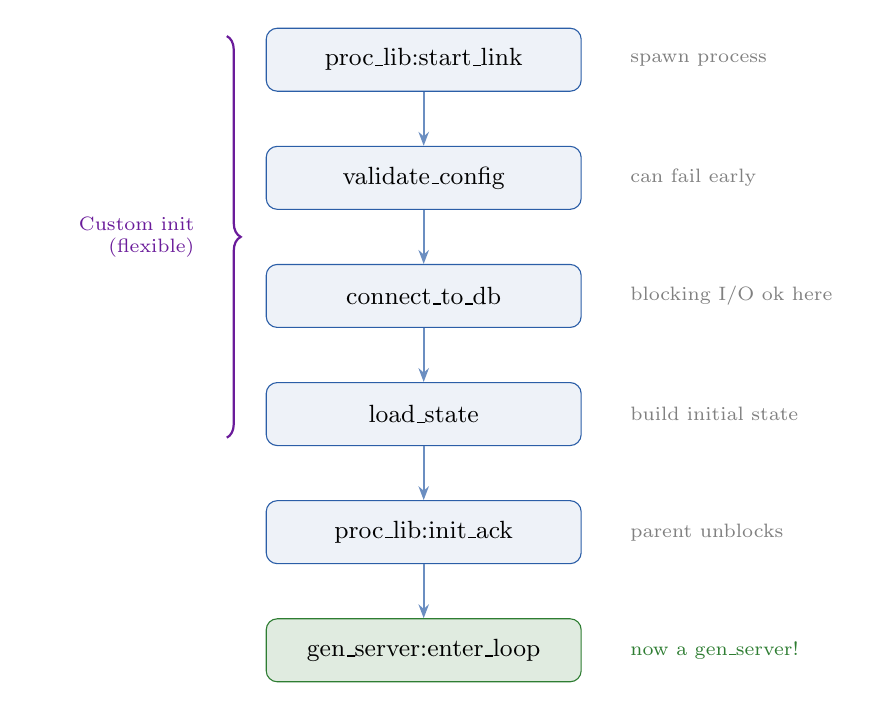
\begin{tikzpicture}[
    stepbox/.style={draw=erlblue, fill=erlblue!8, rounded corners=4pt,
                 minimum width=4cm, minimum height=0.8cm, font=\small},
    arr/.style={-{Stealth[length=5pt]}, thick, erlblue!70},
]
    \node[stepbox] (s1) at (0, 0) {proc\_lib:start\_link};
    \node[stepbox] (s2) at (0, -1.5) {validate\_config};
    \node[stepbox] (s3) at (0, -3) {connect\_to\_db};
    \node[stepbox] (s4) at (0, -4.5) {load\_state};
    \node[stepbox] (s5) at (0, -6) {proc\_lib:init\_ack};
    \node[stepbox, fill=erlgreen!15, draw=erlgreen] (s6) at (0, -7.5) {gen\_server:enter\_loop};

    \draw[arr] (s1) -- (s2);
    \draw[arr] (s2) -- (s3);
    \draw[arr] (s3) -- (s4);
    \draw[arr] (s4) -- (s5);
    \draw[arr] (s5) -- (s6);

    % Annotations
    \node[font=\scriptsize\color{gray}, anchor=west] at (2.5, 0) {spawn process};
    \node[font=\scriptsize\color{gray}, anchor=west] at (2.5, -1.5) {can fail early};
    \node[font=\scriptsize\color{gray}, anchor=west] at (2.5, -3) {blocking I/O ok here};
    \node[font=\scriptsize\color{gray}, anchor=west] at (2.5, -4.5) {build initial state};
    \node[font=\scriptsize\color{gray}, anchor=west] at (2.5, -6) {parent unblocks};
    \node[font=\scriptsize\color{erlgreen}, anchor=west] at (2.5, -7.5) {now a gen\_server!};

    % Brace
    \draw[thick, erlpurple, decorate, decoration={brace, amplitude=5pt}]
        (-2.5, 0.3) -- (-2.5, -4.8)
        node[midway, left=8pt, font=\scriptsize, text width=2cm, align=right] {Custom init\\(flexible)};
\end{tikzpicture}
\caption{enter\_loop 的初始化流程}
\label{fig:enter-loop}
\end{figure}

\begin{warnbox}[重要限制]
\begin{itemize}[leftmargin=1.5em]
    \item 进程\textbf{必须}由 \texttt{proc\_lib} 启动（\texttt{proc\_lib:start\_link}、\texttt{proc\_lib:spawn\_link} 等）
    \item 如果指定了 \texttt{ServerName}，进程必须在调用 \texttt{enter\_loop} 之前已经注册
    \item \texttt{enter\_loop} 永不返回（\texttt{no\_return()}）
\end{itemize}
\end{warnbox}


% ============================================================
% Section 10: handle_continue
% ============================================================
\section{延续处理：handle\_continue/2 (OTP 21+)}

\subsection{动机}

\texttt{init/1} 应该快速返回，不应做耗时操作。但有时初始化后需要做一些后续工作。\texttt{handle\_continue} 提供了一种在 \texttt{init} 返回后、接收任何外部消息之前执行代码的机制。

\begin{lstlisting}[style=erlangstyle, caption={handle\_continue 用法}]
init(Args) ->
    %% Quick init
    State = #{data => undefined},
    %% Schedule continuation BEFORE any external messages
    {ok, State, {continue, load_data}}.

handle_continue(load_data, State) ->
    %% This runs before any call/cast/info
    Data = expensive_load_operation(),
    {noreply, State#{data := Data}, {continue, notify_ready}};

handle_continue(notify_ready, State) ->
    io:format("Server fully initialized~n"),
    {noreply, State}.
\end{lstlisting}

\begin{figure}[H]
\centering
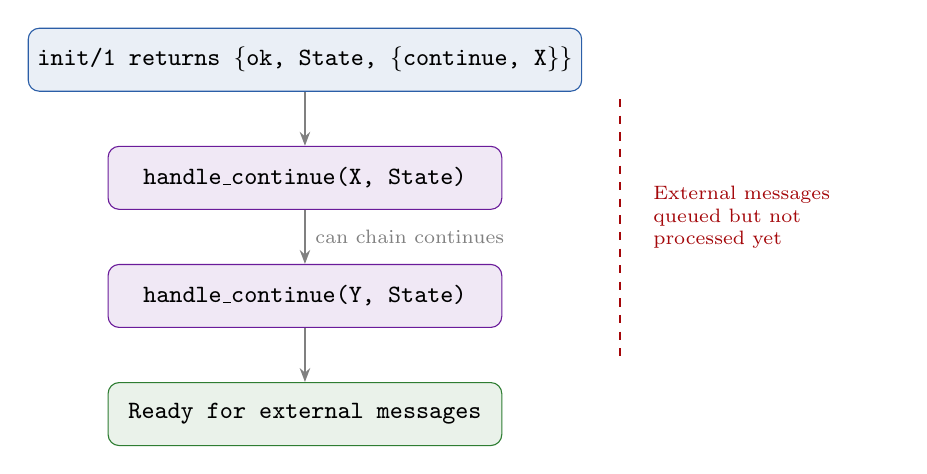
\begin{tikzpicture}[
    phase/.style={draw=#1, fill=#1!10, rounded corners=4pt,
                  minimum width=5cm, minimum height=0.8cm, font=\small\ttfamily},
    arr/.style={-{Stealth[length=5pt]}, thick, gray},
]
    \node[phase=erlblue] (init) at (0, 0) {init/1 returns \{ok, State, \{continue, X\}\}};
    \node[phase=erlpurple] (hc1) at (0, -1.5) {handle\_continue(X, State)};
    \node[phase=erlpurple] (hc2) at (0, -3) {handle\_continue(Y, State)};
    \node[phase=erlgreen] (ready) at (0, -4.5) {Ready for external messages};

    \draw[arr] (init) -- (hc1);
    \draw[arr] (hc1) -- node[right, font=\scriptsize\color{gray}] {can chain continues} (hc2);
    \draw[arr] (hc2) -- (ready);

    % External messages blocked
    \draw[thick, erlred, dashed] (4, -0.5) -- (4, -3.8);
    \node[font=\scriptsize\color{erlred}, anchor=west, text width=3cm] at (4.3, -2) {External messages\\queued but not\\processed yet};
\end{tikzpicture}
\caption{handle\_continue 在外部消息之前执行}
\label{fig:handle-continue}
\end{figure}

\begin{tipbox}[handle\_continue vs 自发消息]
在 OTP 21 之前，常用 \texttt{self() ! post\_init} 来实现类似效果。但这种方式有竞态条件：其他消息可能在 \texttt{post\_init} 之前到达。\texttt{handle\_continue} 保证在任何外部消息之前执行。
\end{tipbox}


% ============================================================
% Section 11: Hibernate
% ============================================================
\section{休眠：hibernate}

\subsection{什么是休眠？}

当 gen\_server 预计会长时间空闲时，可以进入休眠状态。休眠会：
\begin{itemize}[leftmargin=2em]
    \item 触发垃圾回收，释放进程堆内存
    \item 将进程状态压缩到最小
    \item 收到下一条消息时自动唤醒
\end{itemize}

\begin{lstlisting}[style=erlangstyle, caption={休眠的使用方式}]
%% In init
init(Args) ->
    {ok, State, hibernate}.

%% In handle_call
handle_call(Req, _From, State) ->
    {reply, ok, State, hibernate}.

%% In handle_cast
handle_cast(Msg, State) ->
    {noreply, State, hibernate}.

%% In handle_info
handle_info(Info, State) ->
    {noreply, State, hibernate}.
\end{lstlisting}

\subsection{hibernate\_after 选项}

更优雅的方式是使用 \texttt{hibernate\_after} 选项，让 gen\_server 在空闲一段时间后自动休眠：

\begin{lstlisting}[style=shellstyle, caption={hibernate\_after 演示}]
1> {ok, Pid} = gen_server:start(counter_server, 0,
       [{hibernate_after, 3000}]).
{ok,<0.89.0>}

%% Check process info immediately
2> erlang:process_info(Pid, current_function).
{current_function,{gen_server,loop_receive,4}}

%% Wait 3+ seconds, then check again
3> timer:sleep(4000).
ok
4> erlang:process_info(Pid, current_function).
{current_function,{erlang,hibernate,3}}

%% Send a message - wakes up automatically
5> gen_server:call(Pid, get_count).
0
6> erlang:process_info(Pid, current_function).
{current_function,{gen_server,loop_receive,4}}
\end{lstlisting}

\begin{warnbox}[休眠的代价]
休眠涉及至少两次垃圾回收（休眠时和唤醒时）。不要在频繁收到消息的服务器上使用休眠，否则 GC 开销会超过内存节省。
\end{warnbox}


% ============================================================
% Section 12: sys Module Integration
% ============================================================
\section{调试与内省：sys 模块集成}

gen\_server 内置了与 \texttt{sys} 模块的集成，提供强大的运行时调试能力。

\subsection{sys:get\_status/1,2}

\begin{lstlisting}[style=shellstyle, caption={获取服务器状态}]
1> {ok, Pid} = gen_server:start(
       {local, ctr}, counter_server, 0, []).
{ok,<0.89.0>}

2> gen_server:call(ctr, increment).
1
3> gen_server:call(ctr, increment).
2

4> sys:get_status(ctr).
{status,<0.89.0>,
        {module,gen_server},
        [[{"State",#{count => 2, history_length => 2}}],
         ...]}
\end{lstlisting}

\begin{notebox}[format\_status 的作用]
注意输出中 State 显示的是 \texttt{\#\{count => 2, history\_length => 2\}}，而不是完整的 history 列表。这是因为我们实现了 \texttt{format\_status/2}，隐藏了敏感或冗长的数据。
\end{notebox}

\subsection{sys:trace/2 --- 消息追踪}

\begin{lstlisting}[style=shellstyle, caption={开启消息追踪}]
5> sys:trace(ctr, true).
ok

6> gen_server:call(ctr, increment).
*DBG* ctr got call increment from <0.85.0>
*DBG* ctr sent 3 to <0.85.0>, new state #{count => 3,...}
3

7> gen_server:cast(ctr, reset).
*DBG* ctr got cast reset
*DBG* ctr new state #{count => 0,...}
ok

%% Turn off tracing
8> sys:trace(ctr, false).
ok
\end{lstlisting}

\subsection{sys:get\_state/1 和 sys:replace\_state/2}

\begin{lstlisting}[style=shellstyle, caption={直接读取和修改服务器状态}]
%% Get raw state (bypasses format_status)
9> sys:get_state(ctr).
#{count => 0, history => []}

%% Replace state (dangerous! use for debugging only)
10> sys:replace_state(ctr, fun(State) ->
        State#{count := 999}
    end).
#{count => 999, history => []}

11> gen_server:call(ctr, get_count).
999
\end{lstlisting}

\subsection{sys:statistics/2 --- 统计信息}

\begin{lstlisting}[style=shellstyle, caption={收集统计信息}]
12> sys:statistics(ctr, true).
ok

13> gen_server:call(ctr, increment).
1000
14> gen_server:call(ctr, increment).
1001
15> gen_server:cast(ctr, reset).
ok

16> sys:statistics(ctr, get).
{ok,[{start_time,{{2025,4,18},{15,30,0}}},
     {current_time,{{2025,4,18},{15,30,5}}},
     {reductions,156},
     {messages_in,3},
     {messages_out,2}]}

17> sys:statistics(ctr, false).
ok
\end{lstlisting}

\subsection{sys:suspend/1 和 sys:resume/1}

\begin{lstlisting}[style=shellstyle, caption={挂起和恢复服务器}]
%% Suspend - server stops processing messages
18> sys:suspend(ctr).
ok

%% This call will hang (server is suspended)
%% 19> gen_server:call(ctr, get_count, 2000).
%% ** exception exit: {timeout,...}

%% Resume - server processes queued messages
20> sys:resume(ctr).
ok

21> gen_server:call(ctr, get_count).
0
\end{lstlisting}

\subsection{sys 调试工具总览}

\begin{table}[H]
\centering
\small
\begin{tabular}{@{}lp{7cm}@{}}
\toprule
\textbf{函数} & \textbf{说明} \\
\midrule
\texttt{sys:get\_status/1,2} & 获取进程状态（调用 format\_status） \\
\texttt{sys:get\_state/1} & 获取原始 State（不经过 format\_status） \\
\texttt{sys:replace\_state/2} & 替换 State（仅用于调试！） \\
\texttt{sys:trace/2} & 开启/关闭消息追踪 \\
\texttt{sys:statistics/2} & 开启/关闭/获取统计信息 \\
\texttt{sys:suspend/1} & 挂起进程（停止处理消息） \\
\texttt{sys:resume/1} & 恢复进程 \\
\texttt{sys:log/2} & 开启/关闭/获取消息日志 \\
\texttt{sys:log\_to\_file/2} & 将日志写入文件 \\
\bottomrule
\end{tabular}
\caption{sys 模块调试工具}
\end{table}


% ============================================================
% Section 13: Process Registration
% ============================================================
\section{进程注册方式详解}

\subsection{三种注册方式}

\begin{figure}[H]
\centering
\begin{tikzpicture}[scale=0.82, every node/.style={scale=0.82},
    reg/.style={draw=#1, fill=#1!8, rounded corners=6pt,
                minimum width=4.5cm, minimum height=2.5cm, text width=4cm, align=center},
]
    \node[reg=erlblue] (local) at (0, 0) {
        \textbf{\textsf{\{local, Name\}}}\\[4pt]
        \small 当前节点可见\\
        \small \texttt{erlang:register/2}\\
        \small Name 必须是 atom
    };
    \node[reg=erlred] (global) at (5.5, 0) {
        \textbf{\textsf{\{global, Name\}}}\\[4pt]
        \small 所有连接节点可见\\
        \small \texttt{global:register\_name/2}\\
        \small Name 可以是任意 term
    };
    \node[reg=erlpurple] (via) at (11, 0) {
        \textbf{\textsf{\{via, Mod, Name\}}}\\[4pt]
        \small 自定义注册模块\\
        \small 如 gproc, syn\\
        \small 最灵活
    };
\end{tikzpicture}
\caption{三种进程注册方式}
\label{fig:registration}
\end{figure}

\subsection{本地注册}

\begin{lstlisting}[style=shellstyle, caption={本地注册演示}]
1> gen_server:start({local, my_ctr}, counter_server, 0, []).
{ok,<0.89.0>}

%% Access by name
2> gen_server:call(my_ctr, increment).
1

%% whereis finds locally registered processes
3> whereis(my_ctr).
<0.89.0>

%% Cannot register same name twice
4> gen_server:start({local, my_ctr}, counter_server, 0, []).
{error,{already_started,<0.89.0>}}
\end{lstlisting}

\subsection{全局注册}

\begin{lstlisting}[style=shellstyle, caption={全局注册演示}]
5> gen_server:start({global, global_ctr}, counter_server, 0, []).
{ok,<0.95.0>}

%% Access by global name
6> gen_server:call({global, global_ctr}, increment).
1

%% global:whereis_name finds globally registered processes
7> global:whereis_name(global_ctr).
<0.95.0>
\end{lstlisting}

\subsection{不注册（匿名）}

\begin{lstlisting}[style=shellstyle, caption={匿名启动 --- 可以启动多个实例}]
8> {ok, P1} = gen_server:start(counter_server, 0, []).
{ok,<0.100.0>}
9> {ok, P2} = gen_server:start(counter_server, 0, []).
{ok,<0.102.0>}
10> {ok, P3} = gen_server:start(counter_server, 0, []).
{ok,<0.104.0>}

%% Each has independent state
11> gen_server:call(P1, increment).
1
12> gen_server:call(P2, increment).
1
13> gen_server:call(P1, increment).
2
14> gen_server:call(P2, get_count).
1
\end{lstlisting}


% ============================================================
% Section 14: Error Handling
% ============================================================
\section{错误处理与进程链接}

\subsection{trap\_exit 与 EXIT 消息}

\begin{lstlisting}[style=shellstyle, caption={trap\_exit 演示}]
1> {ok, Pid} = gen_server:start(counter_server, 0, []).
{ok,<0.89.0>}

%% counter_server sets trap_exit in init/1
%% So EXIT signals become messages to handle_info

%% Link a process to the server, then kill it
2> Worker = spawn_link(fun() -> timer:sleep(1000) end).
<0.91.0>

%% Link server to worker
3> link(Pid).
true

%% Kill the worker
4> exit(Worker, kill).
true
%% Server receives EXIT message via handle_info:
[counter] linked process <0.91.0> exited: killed
\end{lstlisting}

\subsection{服务器崩溃行为}

\begin{figure}[H]
\centering
\begin{tikzpicture}[
    scenario/.style={draw=#1, fill=#1!5, rounded corners=6pt,
                     minimum width=6cm, minimum height=3cm, text width=5.5cm},
]
    % start_link scenario
    \node[scenario=erlred] (sl) at (0, 0) {};
    \node[font=\bfseries\color{erlred}, anchor=north] at (sl.north) {start\_link + crash};
    \node[font=\small, text width=5cm, align=left] at (0, -0.5) {
        \texttt{1> \{ok,P\} = start\_link().}\\
        \texttt{2> crash(P).}\\
        \texttt{3> self().}\\
        \texttt{<0.88.0>} \textcolor{erlred}{$\leftarrow$ changed!}\\[2pt]
        Shell 也崩溃并重启了
    };

    % start scenario
    \node[scenario=erlgreen] (s) at (8, 0) {};
    \node[font=\bfseries\color{erlgreen}, anchor=north] at (s.north) {start + crash};
    \node[font=\small, text width=5cm, align=left] at (8, -0.5) {
        \texttt{1> \{ok,P\} = start().}\\
        \texttt{2> crash(P).}\\
        \texttt{3> self().}\\
        \texttt{<0.85.0>} \textcolor{erlgreen}{$\leftarrow$ unchanged}\\[2pt]
        Shell 不受影响
    };
\end{tikzpicture}
\caption{start\_link vs start 在服务器崩溃时的行为差异}
\label{fig:crash-behavior}
\end{figure}

\subsection{catch 保护 call}

\begin{lstlisting}[style=erlangstyle, caption={安全地调用可能崩溃的服务器}]
%% Using try-catch to handle server crashes
safe_call(Server, Request) ->
    try gen_server:call(Server, Request) of
        Result -> {ok, Result}
    catch
        exit:{noproc, _} ->
            {error, server_not_running};
        exit:{timeout, _} ->
            {error, timeout};
        exit:{normal, _} ->
            {error, server_stopped};
        exit:{Reason, _} ->
            {error, {server_crashed, Reason}}
    end.
\end{lstlisting}


% ============================================================
% Section 15: format_status
% ============================================================
\section{状态格式化：format\_status}

\subsection{为什么需要 format\_status？}

当 gen\_server 崩溃时，OTP 会生成 crash report，其中包含完整的 State。如果 State 中包含敏感信息（密码、token）或大量数据，这些都会出现在日志中。

\begin{lstlisting}[style=erlangstyle, caption={format\_status/2 回调（OTP 25 之前）}]
%% Called by sys:get_status and crash reports
format_status(_Opt, [_PDict, State]) ->
    %% Return sanitized state for display
    [{data, [{"State", sanitize(State)}]}].

sanitize(#{password := _, token := _} = State) ->
    State#{password := "***", token := "***"}.
\end{lstlisting}

\begin{lstlisting}[style=erlangstyle, caption={format\_status/1 回调（OTP 25+，新格式）}]
%% New format_status/1 (OTP 25+)
format_status(Status) ->
    Status#{state := sanitize(maps:get(state, Status))}.
\end{lstlisting}

\begin{lstlisting}[style=shellstyle, caption={format\_status 效果对比}]
%% Without format_status:
1> sys:get_state(server).
#{count => 42, history => [{inc,42},{inc,41},...100 items...]}

%% With format_status:
2> sys:get_status(server).
{status,...,[{"State", #{count => 42, history_length => 100}}],...}
\end{lstlisting}


% ============================================================
% Section 16: code_change
% ============================================================
\section{热代码升级：code\_change/3}

\subsection{概述}

Erlang 支持在不停止系统的情况下升级代码。当 gen\_server 的 State 数据结构发生变化时，\texttt{code\_change/3} 负责将旧的 State 迁移为新格式。

\begin{lstlisting}[style=erlangstyle, caption={code\_change/3 回调}]
code_change(OldVsn, OldState, Extra) ->
    {ok, NewState}.

%% OldVsn: version from -vsn attribute, or {down, Vsn} for downgrade
%% Extra:  from .appup file
\end{lstlisting}

\begin{lstlisting}[style=erlangstyle, caption={code\_change 示例：State 从 tuple 迁移到 map}]
%% Old state: {Count, History}
%% New state: #{count => Count, history => History}

code_change("1.0", {Count, History}, _Extra) ->
    NewState = #{count => Count, history => History},
    {ok, NewState};
code_change(_OldVsn, State, _Extra) ->
    {ok, State}.
\end{lstlisting}

\begin{notebox}[实际使用]
热代码升级在实际生产中使用较少（大多数团队选择滚动重启）。但理解 \texttt{code\_change} 有助于理解 OTP 的设计哲学：系统应该能够在不停机的情况下演进。
\end{notebox}


% ============================================================
% Section 17: Complete API Reference
% ============================================================
\section{API 完整参考}

\subsection{启动函数}

\begin{table}[H]
\centering
\small
\begin{tabular}{@{}lp{7cm}@{}}
\toprule
\textbf{函数} & \textbf{说明} \\
\midrule
\texttt{start/3,4} & 启动，不链接 \\
\texttt{start\_link/3,4} & 启动并链接（生产环境） \\
\texttt{start\_monitor/3,4} & 启动并监控（OTP 23+） \\
\texttt{enter\_loop/3,4,5} & 将已有进程变为 gen\_server \\
\bottomrule
\end{tabular}
\caption{启动函数}
\end{table}

\subsection{请求函数}

\begin{table}[H]
\centering
\small
\begin{tabular}{@{}lp{7cm}@{}}
\toprule
\textbf{函数} & \textbf{说明} \\
\midrule
\texttt{call/2,3} & 同步调用（阻塞，默认 5s 超时） \\
\texttt{cast/2} & 异步调用（fire \& forget） \\
\texttt{send\_request/2} & 异步发送请求，返回 ReqId（OTP 23+） \\
\texttt{send\_request/4} & 异步发送请求到集合（OTP 25+） \\
\texttt{reply/2} & 显式回复 call 请求 \\
\bottomrule
\end{tabular}
\caption{请求函数}
\end{table}

\subsection{响应收取函数}

\begin{table}[H]
\centering
\small
\begin{tabular}{@{}lp{7cm}@{}}
\toprule
\textbf{函数} & \textbf{说明} \\
\midrule
\texttt{receive\_response/2,3} & 阻塞等待回复，清理残留消息 \\
\texttt{wait\_response/2,3} & 阻塞等待回复，不清理残留消息 \\
\texttt{check\_response/2,3} & 非阻塞检查回复 \\
\texttt{reqids\_new/0} & 创建请求 ID 集合 \\
\texttt{reqids\_size/1} & 获取集合中待处理请求数 \\
\texttt{reqids\_add/3} & 向集合添加请求 ID \\
\texttt{reqids\_to\_list/1} & 将集合转为列表 \\
\bottomrule
\end{tabular}
\caption{响应收取函数（OTP 23+）}
\end{table}

\subsection{多节点函数}

\begin{table}[H]
\centering
\small
\begin{tabular}{@{}lp{7cm}@{}}
\toprule
\textbf{函数} & \textbf{说明} \\
\midrule
\texttt{multi\_call/2,3,4} & 并行同步调用多个节点 \\
\texttt{abcast/2,3} & 并行异步广播到多个节点 \\
\bottomrule
\end{tabular}
\caption{多节点函数}
\end{table}

\subsection{生命周期函数}

\begin{table}[H]
\centering
\small
\begin{tabular}{@{}lp{7cm}@{}}
\toprule
\textbf{函数} & \textbf{说明} \\
\midrule
\texttt{stop/1,3} & 优雅停止服务器 \\
\bottomrule
\end{tabular}
\caption{生命周期函数}
\end{table}

\subsection{回调函数}

\begin{table}[H]
\centering
\small
\begin{tabular}{@{}lp{7cm}@{}}
\toprule
\textbf{回调} & \textbf{触发时机} \\
\midrule
\texttt{init/1} & 进程启动时 \\
\texttt{handle\_call/3} & 收到 call 请求 \\
\texttt{handle\_cast/2} & 收到 cast 请求 \\
\texttt{handle\_info/2} & 收到其他消息 \\
\texttt{handle\_continue/2} & 上一个回调返回 \texttt{\{continue, ...\}} \\
\texttt{terminate/2} & 进程即将终止 \\
\texttt{code\_change/3} & 热代码升级 \\
\texttt{format\_status/1,2} & sys:get\_status 或 crash report \\
\bottomrule
\end{tabular}
\caption{回调函数}
\end{table}

\subsection{API 全景图}

\begin{figure}[H]
\centering
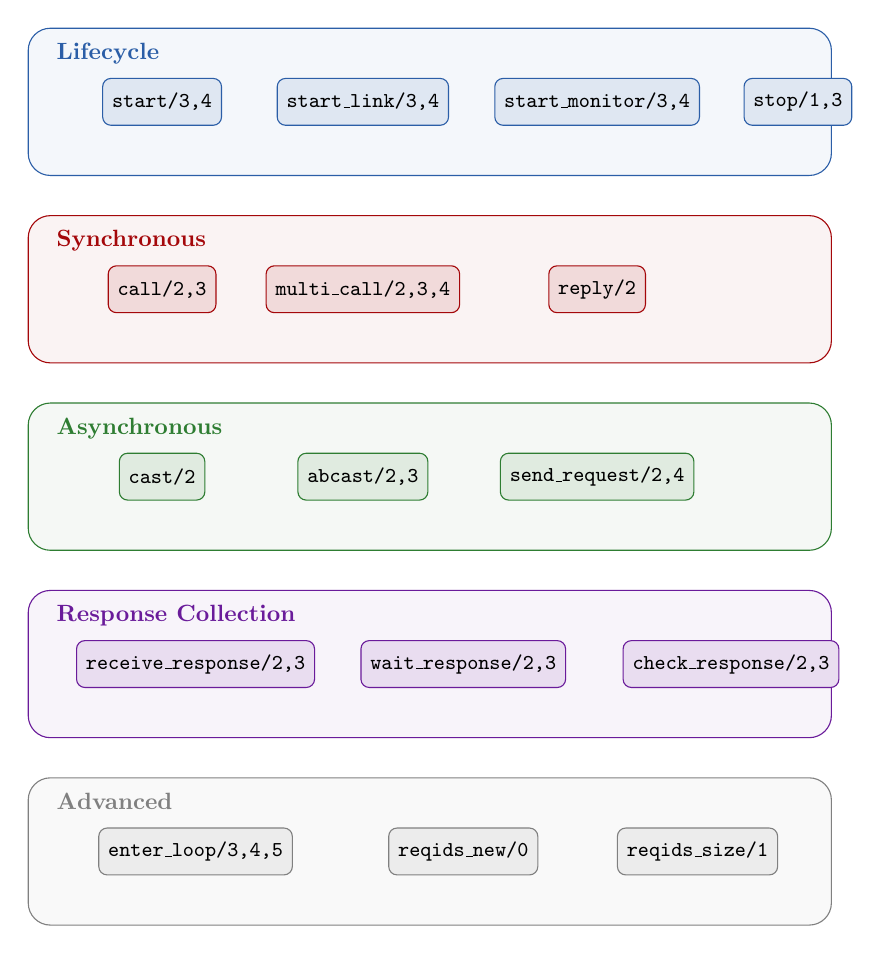
\begin{tikzpicture}[scale=0.85, every node/.style={scale=0.85},
    group/.style={draw=#1, fill=#1!5, rounded corners=8pt, inner sep=10pt},
    api/.style={draw=#1, fill=#1!15, rounded corners=3pt,
                minimum height=0.7cm, font=\small\ttfamily, inner sep=4pt},
]
    % Lifecycle group
    \node[group=erlblue, minimum width=12cm, minimum height=2.2cm] (lg) at (6, 8) {};
    \node[font=\bfseries\color{erlblue}, anchor=north west] at (0.3, 9) {Lifecycle};
    \node[api=erlblue] at (2, 8) {start/3,4};
    \node[api=erlblue] at (5, 8) {start\_link/3,4};
    \node[api=erlblue] at (8.5, 8) {start\_monitor/3,4};
    \node[api=erlblue] at (11.5, 8) {stop/1,3};

    % Sync group
    \node[group=erlred, minimum width=12cm, minimum height=2.2cm] (sg) at (6, 5.2) {};
    \node[font=\bfseries\color{erlred}, anchor=north west] at (0.3, 6.2) {Synchronous};
    \node[api=erlred] at (2, 5.2) {call/2,3};
    \node[api=erlred] at (5, 5.2) {multi\_call/2,3,4};
    \node[api=erlred] at (8.5, 5.2) {reply/2};

    % Async group
    \node[group=erlgreen, minimum width=12cm, minimum height=2.2cm] (ag) at (6, 2.4) {};
    \node[font=\bfseries\color{erlgreen}, anchor=north west] at (0.3, 3.4) {Asynchronous};
    \node[api=erlgreen] at (2, 2.4) {cast/2};
    \node[api=erlgreen] at (5, 2.4) {abcast/2,3};
    \node[api=erlgreen] at (8.5, 2.4) {send\_request/2,4};

    % Response group
    \node[group=erlpurple, minimum width=12cm, minimum height=2.2cm] (rg) at (6, -0.4) {};
    \node[font=\bfseries\color{erlpurple}, anchor=north west] at (0.3, 0.6) {Response Collection};
    \node[api=erlpurple] at (2.5, -0.4) {receive\_response/2,3};
    \node[api=erlpurple] at (6.5, -0.4) {wait\_response/2,3};
    \node[api=erlpurple] at (10.5, -0.4) {check\_response/2,3};

    % Advanced group
    \node[group=gray, minimum width=12cm, minimum height=2.2cm] (adg) at (6, -3.2) {};
    \node[font=\bfseries\color{gray}, anchor=north west] at (0.3, -2.2) {Advanced};
    \node[api=gray] at (2.5, -3.2) {enter\_loop/3,4,5};
    \node[api=gray] at (6.5, -3.2) {reqids\_new/0};
    \node[api=gray] at (10, -3.2) {reqids\_size/1};
\end{tikzpicture}
\caption{gen\_server API 全景图}
\label{fig:api-overview}
\end{figure}


% ============================================================
% Section 18: Common Pitfalls
% ============================================================
\section{常见陷阱与最佳实践}

\subsection{陷阱 1：在 handle\_call 中调用自己}

\begin{lstlisting}[style=erlangstyle, caption={死锁！}]
handle_call(request1, _From, State) ->
    %% DEADLOCK: gen_server is single-process,
    %% it cannot process request2 while handling request1
    Result = gen_server:call(self(), request2),
    {reply, Result, State}.
\end{lstlisting}

\begin{figure}[H]
\centering
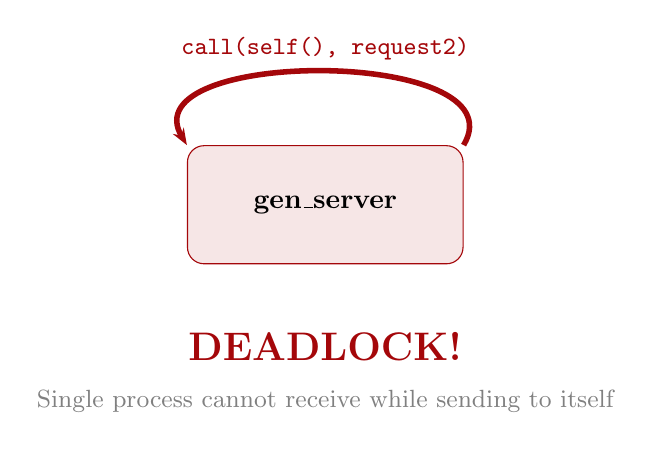
\begin{tikzpicture}
    \node[draw=erlred, fill=erlred!10, rounded corners=6pt,
          minimum width=3.5cm, minimum height=1.5cm, font=\bfseries] (gs) at (0,0) {gen\_server};

    \draw[-{Stealth[length=6pt]}, thick, erlred, line width=2pt]
        (gs.north east) .. controls (2.5, 2) and (-2.5, 2) .. (gs.north west)
        node[midway, above, font=\small\ttfamily] {call(self(), request2)};

    \node[font=\Large\bfseries\color{erlred}] at (0, -1.8) {DEADLOCK!};
    \node[font=\small\color{gray}] at (0, -2.5) {Single process cannot receive while sending to itself};
\end{tikzpicture}
\caption{gen\_server 调用自己导致死锁}
\end{figure}

\subsection{陷阱 2：cast 没有背压}

\begin{lstlisting}[style=erlangstyle, caption={cast 导致消息队列爆炸}]
%% BAD: Flooding server with casts
lists:foreach(fun(I) ->
    gen_server:cast(Server, {process, I})
end, lists:seq(1, 1000000)).
%% Server's message queue grows to 1M messages!

%% BETTER: Use call for back-pressure
lists:foreach(fun(I) ->
    gen_server:call(Server, {process, I})
end, lists:seq(1, 1000000)).
%% Each call waits for server to finish before sending next
\end{lstlisting}

\subsection{陷阱 3：忘记处理未知消息}

\begin{lstlisting}[style=erlangstyle, caption={总是添加 catch-all 子句}]
%% BAD: Missing catch-all
handle_info({expected_msg, Data}, State) ->
    {noreply, handle_data(Data, State)}.
%% Unknown messages cause crash!

%% GOOD: With catch-all
handle_info({expected_msg, Data}, State) ->
    {noreply, handle_data(Data, State)};
handle_info(Unknown, State) ->
    logger:warning("Unexpected message: ~p", [Unknown]),
    {noreply, State}.
\end{lstlisting}

\subsection{陷阱 4：init/1 中做耗时操作}

\begin{lstlisting}[style=erlangstyle, caption={init 中的耗时操作会阻塞调用者}]
%% BAD: Blocks the caller of start_link
init(Args) ->
    Data = load_huge_dataset(),  %% Takes 30 seconds!
    {ok, Data}.

%% GOOD: Use handle_continue
init(Args) ->
    {ok, #{data => undefined}, {continue, load_data}}.

handle_continue(load_data, State) ->
    Data = load_huge_dataset(),
    {noreply, State#{data := Data}}.
\end{lstlisting}

\subsection{最佳实践总结}

\begin{table}[H]
\centering
\small
\begin{tabular}{@{}cp{10cm}@{}}
\toprule
\textbf{\#} & \textbf{实践} \\
\midrule
1 & 生产环境始终使用 \texttt{start\_link}，配合 supervisor \\
2 & 保持 \texttt{handle\_call} 快速（默认 5s 超时） \\
3 & 需要返回值或确认时用 \texttt{call}，否则用 \texttt{cast} \\
4 & 所有 \texttt{handle\_*} 回调都添加 catch-all 子句 \\
5 & 用 \texttt{handle\_continue} 代替 \texttt{init} 中的耗时操作 \\
6 & 用 \texttt{format\_status} 隐藏敏感信息 \\
7 & 不要在 \texttt{handle\_call} 中 \texttt{call} 自己（\texttt{gen\_server:call(self(), ...)} 会死锁） \\
8 & 大量请求时用 \texttt{call}（背压）而非 \texttt{cast} \\
9 & 长时间空闲的服务器使用 \texttt{hibernate\_after} \\
10 & 需要并行请求多个服务器时用 \texttt{send\_request} \\
\bottomrule
\end{tabular}
\caption{gen\_server 最佳实践}
\end{table}


\end{document}
